\documentclass[journal,twoside,web]{ieeecolor}
\usepackage{generic}
\usepackage{cite}
\usepackage{amsmath,amssymb,amsfonts}
\usepackage{algorithmic}
\usepackage{graphicx}
\usepackage{textcomp}
\usepackage{array}
\newcolumntype{L}[1]{>{\raggedright\let\newline\\\arraybackslash\hspace{0pt}}m{#1}}
\newcolumntype{C}[1]{>{\centering\let\newline\\\arraybackslash\hspace{0pt}}m{#1}}
\newcolumntype{R}[1]{>{\raggedleft\let\newline\\\arraybackslash\hspace{0pt}}m{#1}}
\def\BibTeX{{\rm B\kern-.05em{\sc i\kern-.025em b}\kern-.08em
    T\kern-.1667em\lower.7ex\hbox{E}\kern-.125emX}}
\markboth{\journalname, VOL. XX, NO. XX, XXXX 2023}
{Author \MakeLowercase{\textit{et al.}}: Short Wave Infrared Neuromodulation Gadget (May 2023)}
\begin{document}
\title{Short Wave Infrared Neuromodulation Gadget (May 2023)}
\author{Cameron R. Author, \IEEEmembership{Member, IEEE}, Matthew T. Author, Bibhus L. Author, 
        Krishna S. Sponsor, \IEEEmembership{Member, IEEE}, John L. Mentor, \IEEEmembership{Member, IEEE}
\thanks{ }
\thanks{ }
\thanks{ }
\thanks{ }}

\maketitle

\begin{abstract}
    Direct stimulation of neurons in the brain can potentially treat many diseases, such as Parkinson's  
    or Alzheimer's disease. Direct stimulation, whether it be through electric or photonic stimulation,  
    provided a way to activate neurons in the brain and treat diseases and conditions. However, this kind  
    of invasive stimulation can have risks that lead to worsening the condition or cause infection.  
    The Short-Wave Infrared Neuromodulation Gadget (SWING) aimed to build and test a non-invasive optical method  
    of stimulation with funding provided by the KIND Laboratory's Brain IMPACT project. SWING is part of the  
    two semester long Electrical and Computer Engineering capstone sequence at The Ohio State University. 
    
    Because the optical coefficients of biological tissue are not well known at 1550 nm,  
    SWING used a cubic extrapolation to approximate these coefficients. Monte Carlo eXtreme (MCX) was then used to predict the  
    expected photon distribution and intensity throughout a model of the human head. MCX was ran multiple times with different positions 
    and wavelengths using The Ohio State Supercomputer. MCX showed that deep brain stimulation is possible at all the wavelengths tested. 
    Based on the MCX results, 1550nm wavelength is the best choice for further testing. Solving the problems previously discussed has the 
    potential to reduce the effects of brain disorders on the general population, mitigate the risks of surgery that patients would have to 
    go through if done invasively, and to improve overall health. 
\end{abstract}

\begin{IEEEkeywords}

\end{IEEEkeywords}

\section{Introduction}
\label{sec:introduction}
There are many physical issues in the brain, including Parkinson's disease and functional problems such as attention-deficit/hyperactivity disorder (ADHD)  
and depressive disorders. A solution to such problems that has been explored recently in the Neurotech community is one that involves a direct stimulation of  
neuronal connections in the brain [1]. Direct neuronal stimulation, whether it be through electric or photonic stimulation, provides a way to control  
mechanisms in the brain and treat diseases and conditions. These treatments result in an improvement of the effects caused by these diseases and conditions.  
However, most modern neuromodulation strategies are invasive in nature, and there are limited options for a non-invasive approach to neuromodulation for medical benefit.  
Many invasive techniques involve surgical implants and increase the risk of brain hemorrhage and worsening mental and emotional status for some patients,  
that often make the cons worse for life-threatening conditions [1]. As a result, SWING looks to investigate a non-invasive method for neuromodulation  
using a near-infrared photonic stimulation method. 


\section{Methods}
\label{sec:methods}
SWING's software and simulation consisted of two main components: software for data preprocessing and simulation for modeling and photon distribution. 
The preprocessing stage involved approximating optical coefficients at 1550 nm.. Monte Carlo eXtreme (MCX) is used for simulating the 
behavior of the laser as it scatters and is absorbed through the Optical Phantom head, providing a model of photon dispersion in biological tissue using known or 
approximated optical coefficients.

\subsection{Software Preprocessing}
In the software preprocessing stage, the model approximated the optical coefficients of layers in the brain where it is unknown for 1550nm sources. Optical coefficient data for the scalp, skull, gray matter (GM), and white matter (WM) are obtained from [SOURCE]. The wavelength ranges for each layer are as follows: scalp (805-2000 nm), 
skull (801-2000 nm), gray matter (400-1300 nm), and white matter (400-1300 nm). The data for scalp and skull cover the wavelength of interest (1550 nm), but the data 
for GM and WM do not. To address this, cubic extrapolation and interpolation methods are used to process the data and extrapolate the unknown layers to 1550nm. 

The cubic interpolation method approximates the optical coefficients for the gray matter (GM) and white matter (WM) layers at 1550 nm based on the known data points. Let $x$ represent the wavelength and $y$ represent the absorption coefficient. The cubic interpolation function can be defined as follows:

\[
y(x) = a(x-x_1)^3 + b(x-x_1)^2 + c(x-x_1) + d
\]

where $(x_1, y_1)$, $(x_2, y_2)$, $(x_3, y_3)$, and $(x_4, y_4)$ are the known data points for a specific layer (GM or WM).

To determine the coefficients $a$, $b$, $c$, and $d$, the model solves the following system of equations using the known data points:

\[
\begin{aligned}
y_1 &= a(x_1-x_1)^3 + b(x_1-x_1)^2 + c(x_1-x_1) + d \\
y_2 &= a(x_2-x_1)^3 + b(x_2-x_1)^2 + c(x_2-x_1) + d \\
y_3 &= a(x_3-x_1)^3 + b(x_3-x_1)^2 + c(x_3-x_1) + d \\
y_4 &= a(x_4-x_1)^3 + b(x_4-x_1)^2 + c(x_4-x_1) + d \\
\end{aligned}
\]

Solving this system of equations provides the coefficients $a$, $b$, $c$, and $d$ specific to the cubic interpolation for the respective layer.

To apply the cubic interpolation in this study, Python programming language was used to process the known data points and calculate the coefficients. Once the coefficients are obtained, the cubic interpolation function is used to estimate the absorption coefficient at any desired wavelength within the range. This cubic interpolation provides a complex fit while preventing over-fitting in the initial steps. This allows extrapolation of the gray and white matter absorption coefficients to 1550 nm within the overlapping region (801-1300 nm), providing continuous lines for the unknown layers.

To extrapolate the optical coefficients of the gray matter (GM) and white matter (WM) layers to 1550 nm, the overlapping region of the four tissues (801-1300 nm) is examined. Vertical offset values between the unknown layers (GM and WM) and the known layers (scalp and skull) are calculated throughout this overlapping region.

Let \( \lambda \) represent the wavelength and \( \mu \) represent the absorption coefficient. The vertical offset values can be calculated as the difference between the absorption coefficients of the unknown layers and the known layers at each wavelength in the overlapping region. These offset values are averaged to obtain two average vertical offsets, one for each unknown layer. Let \( \text{AvgOffsetGM} \) represent the average vertical offset of the gray matter, and \( \text{AvgOffsetWM} \) represent the average vertical offset of the white matter. The extrapolation model then extends the unknown layers by adding the previously calculated offsets to the known scalp and skull data.

The average vertical offsets of the gray matter and white matter can be expressed as:

$$
\text{AvgOffsetGM} = \frac{1}{N} \sum_{i=1}^{N} (\mu_{\text{GM,unknown}}(\lambda_i) - \mu_{\text{GM,known}}(\lambda_i))
$$
$$
\text{AvgOffsetWM} = \frac{1}{N} \sum_{i=1}^{N} (\mu_{\text{WM,unknown}}(\lambda_i) - \mu_{\text{WM,known}}(\lambda_i))
$$

where \( N \) represents the number of data points within the overlapping region, \( \mu_{\text{GM,unknown}}(\lambda_i) \) and \( \mu_{\text{WM,unknown}}(\lambda_i) \) denote the absorption coefficients of the unknown layers at the \( i \)-th wavelength, and \( \mu_{\text{GM,known}}(\lambda_i) \) and \( \mu_{\text{WM,known}}(\lambda_i) \) denote the absorption coefficients of the known layers at the \( i \)-th wavelength.

In this study, Python programming language was used to process the absorption coefficient data and calculate the vertical offset values. The following equations were used to perform the extrapolation:

\[
\mu_{\text{GM,extrapolated}}(\lambda) = \mu_{\text{GM,known}}(\lambda) + \text{AvgOffsetGM}
\]
\[
\mu_{\text{WM,extrapolated}}(\lambda) = \mu_{\text{WM,known}}(\lambda) + \text{AvgOffsetWM}
\]

To ensure accuracy and account for variations, this process of calculating vertical offsets and performing extrapolation is repeated for multiple data points within the overlapping region.

Figures 7, 8, and 9 visualize the results of the extrapolation process. Figure 7 shows the overlapping region of absorption coefficients, and Figures 8 and 9 display the extrapolated absorption coefficients at 1550 nm. These figures, generated using Python, provide a graphical representation of the extrapolation results and aid in understanding the estimated optical coefficients of the GM and WM layers at the wavelength of interest.

% By applying this cubic interpolation method to the known data points using Python, continuous curves are generated for the optical coefficients of the gray matter and white matter layers. These curves provide an estimation of the absorption coefficients at the wavelength of interest, facilitating further analysis and simulation in the TIRE project.


% First, known data points are plotted, and a cubic interpolation is applied between each point to obtain continuous lines for the four biological tissue layers. 
% This cubic interpolation provides a complex fit while preventing over-fitting in the initial steps. To extrapolate the gray and white matter to 1550 nm, the overlapping 
% region of the four tissues (801-1300 nm) is examined.

% Vertical offset values between the unknown layers (gray matter and white matter) and the known layers (scalp and skull) are calculated throughout the overlapping region. 
% These offset values are averaged, resulting in two average vertical offsets for each unknown layer. The extrapolation model extends the unknown layers by adding the 
% previously calculated offsets to the known scalp and skull data. This process is repeated to calculate a third extrapolation by taking the average of the scalp and skull 
% extrapolations. The results are visualized in Figures 7, 8, and 9, showing the extrapolated lines and marker denoting the extrapolated values at 1550 nm.

\subsection{Simulation using MCX}
MCX, a Monte Carlo simulation tool, is employed for visualizing the optical intensity and behavior of a laser source within the head and brain tissue. It models the photon dispersion in biological tissue using optical 
coefficients obtained from experimental data or approximations, as in the case of SWING. MCX creates a mesh model of the human brain using an accumulation of MRI images, incorporating layers such as scalp, skull, Cerebral Spinal Fluid (CSF), GM, WM, and air bubbles. Thickness variations in the layers are specified using thinning or thickening operators.
To create the simulation, the optical coefficients, particularly the absorption and scattering coefficients, are input into the MCX software. This allows for the simulation of photon absorption and scattering as light passes through the brain tissue, enabling visualization of beam intensity at different points in the brain.
Additionally, TIRE utilizes the software to investigate various aspects of photon dispersion. This includes studying the impact of different tissue layers on beam intensity and exploring the effects of laser parameters such as wavelength, illumination area size, and the number of incident photons on the phantom.  The differences between absorption coefficients at 1550 nm compared to other wavelength be observed and noted in the figures, and this model can be utilized for experimental data validation.



\section{Results}
\label{sec:results}

Table ~\ref{CoefficientTable} below displays the estimated absorption and scattering coefficients for each of the biological tissue layers as well as each wavelength.
These values were calculated using the interpolation-extrapolation method detailed in ~\ref(sec:methods). To determine the reliability of this prediction method, SWING used
the Python library "scikit-learn" to calculate the R-squared value when predicting known data. This R-squared value was calculated as 0.4980, indicating that 49.80\% of the 
variability in the unknown coefficients is explained by SWING's predicition model.

\begin{table}
\centering
\caption{Estimated Optical Coefficients}
\label{CoefficientTable}
\setlength{\tabcolsep}{3pt}
\renewcommand{\arraystretch}{1.5}
\resizebox{\columnwidth}{!}{%
\begin{tabular}{|L{45pt}|L{60pt}|C{60pt}|C{60pt}|}
\hline
Tissue & Wavelength, nm & Absorption Coefficient $\mu_{a}$, cm$^{-1}$ &  Reduced Scattering Coefficient $\mu_{s}^{'}$, cm$^{-1}$ \\
\hline
Scalp & 810 & 0.505 & 2.35 \\
&       980 & 1.23 & 2.35 \\
&       1064 & 1.23 & 2.35 \\
&       1550 & 1.23 & 2.35 \\
Skull & 810 & 0.099 & 2.35 \\
&       980 & 1.23 & 2.35 \\
&       1064 & 1.23 & 2.35 \\
&       1550 & 1.23 & 2.35 \\
Gray Matter & 810 & 0.455 & 2.35 \\
&       980 & 1.23 & 2.35 \\
&       1064 & 1.23 & 2.35 \\
&       1550 & 1.23 & 2.35 \\
White Matter & 810 & 1.23 & 2.35 \\
&       980 & 1.23 & 2.35 \\
&       1064 & 1.23 & 2.35 \\
&       1550 & 1.23 & 2.35 \\
\hline
\end{tabular}%
}
\label{tab1}
\end{table}

\begin{figure}[!htb]
    \center{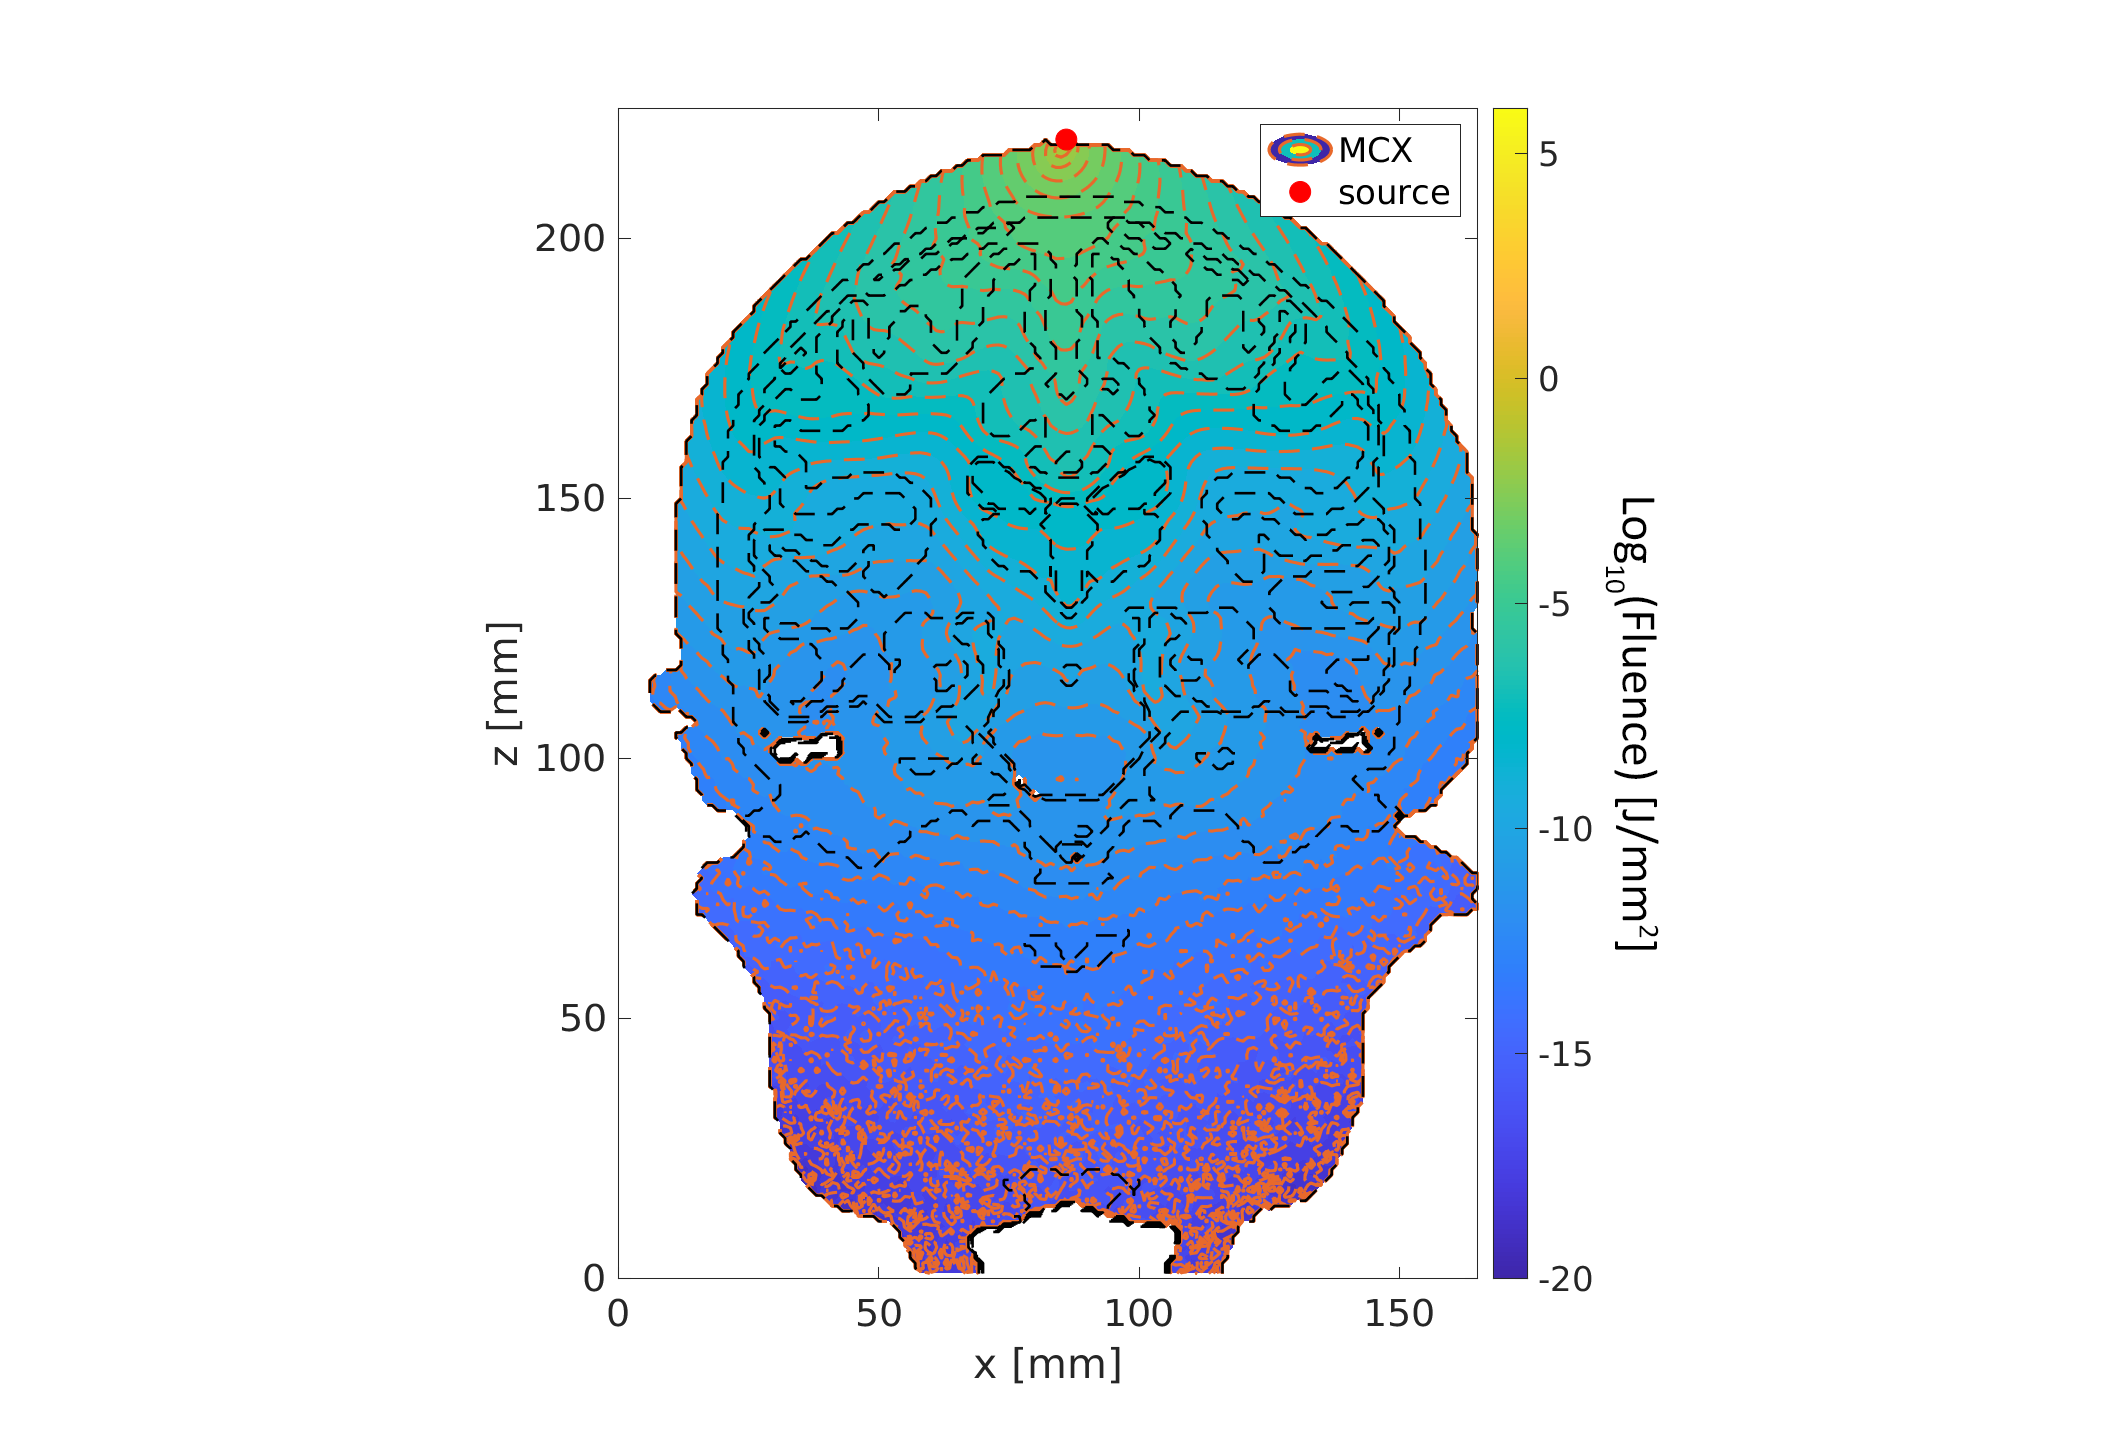
\includegraphics[width=\columnwidth]
    {Figures/Fluence_Distribution_810nm_CZ.png}}
    \caption{\label{fig:810-CZ} 810 nm CZ Position}
\end{figure}

\begin{figure}[!htb]
    \center{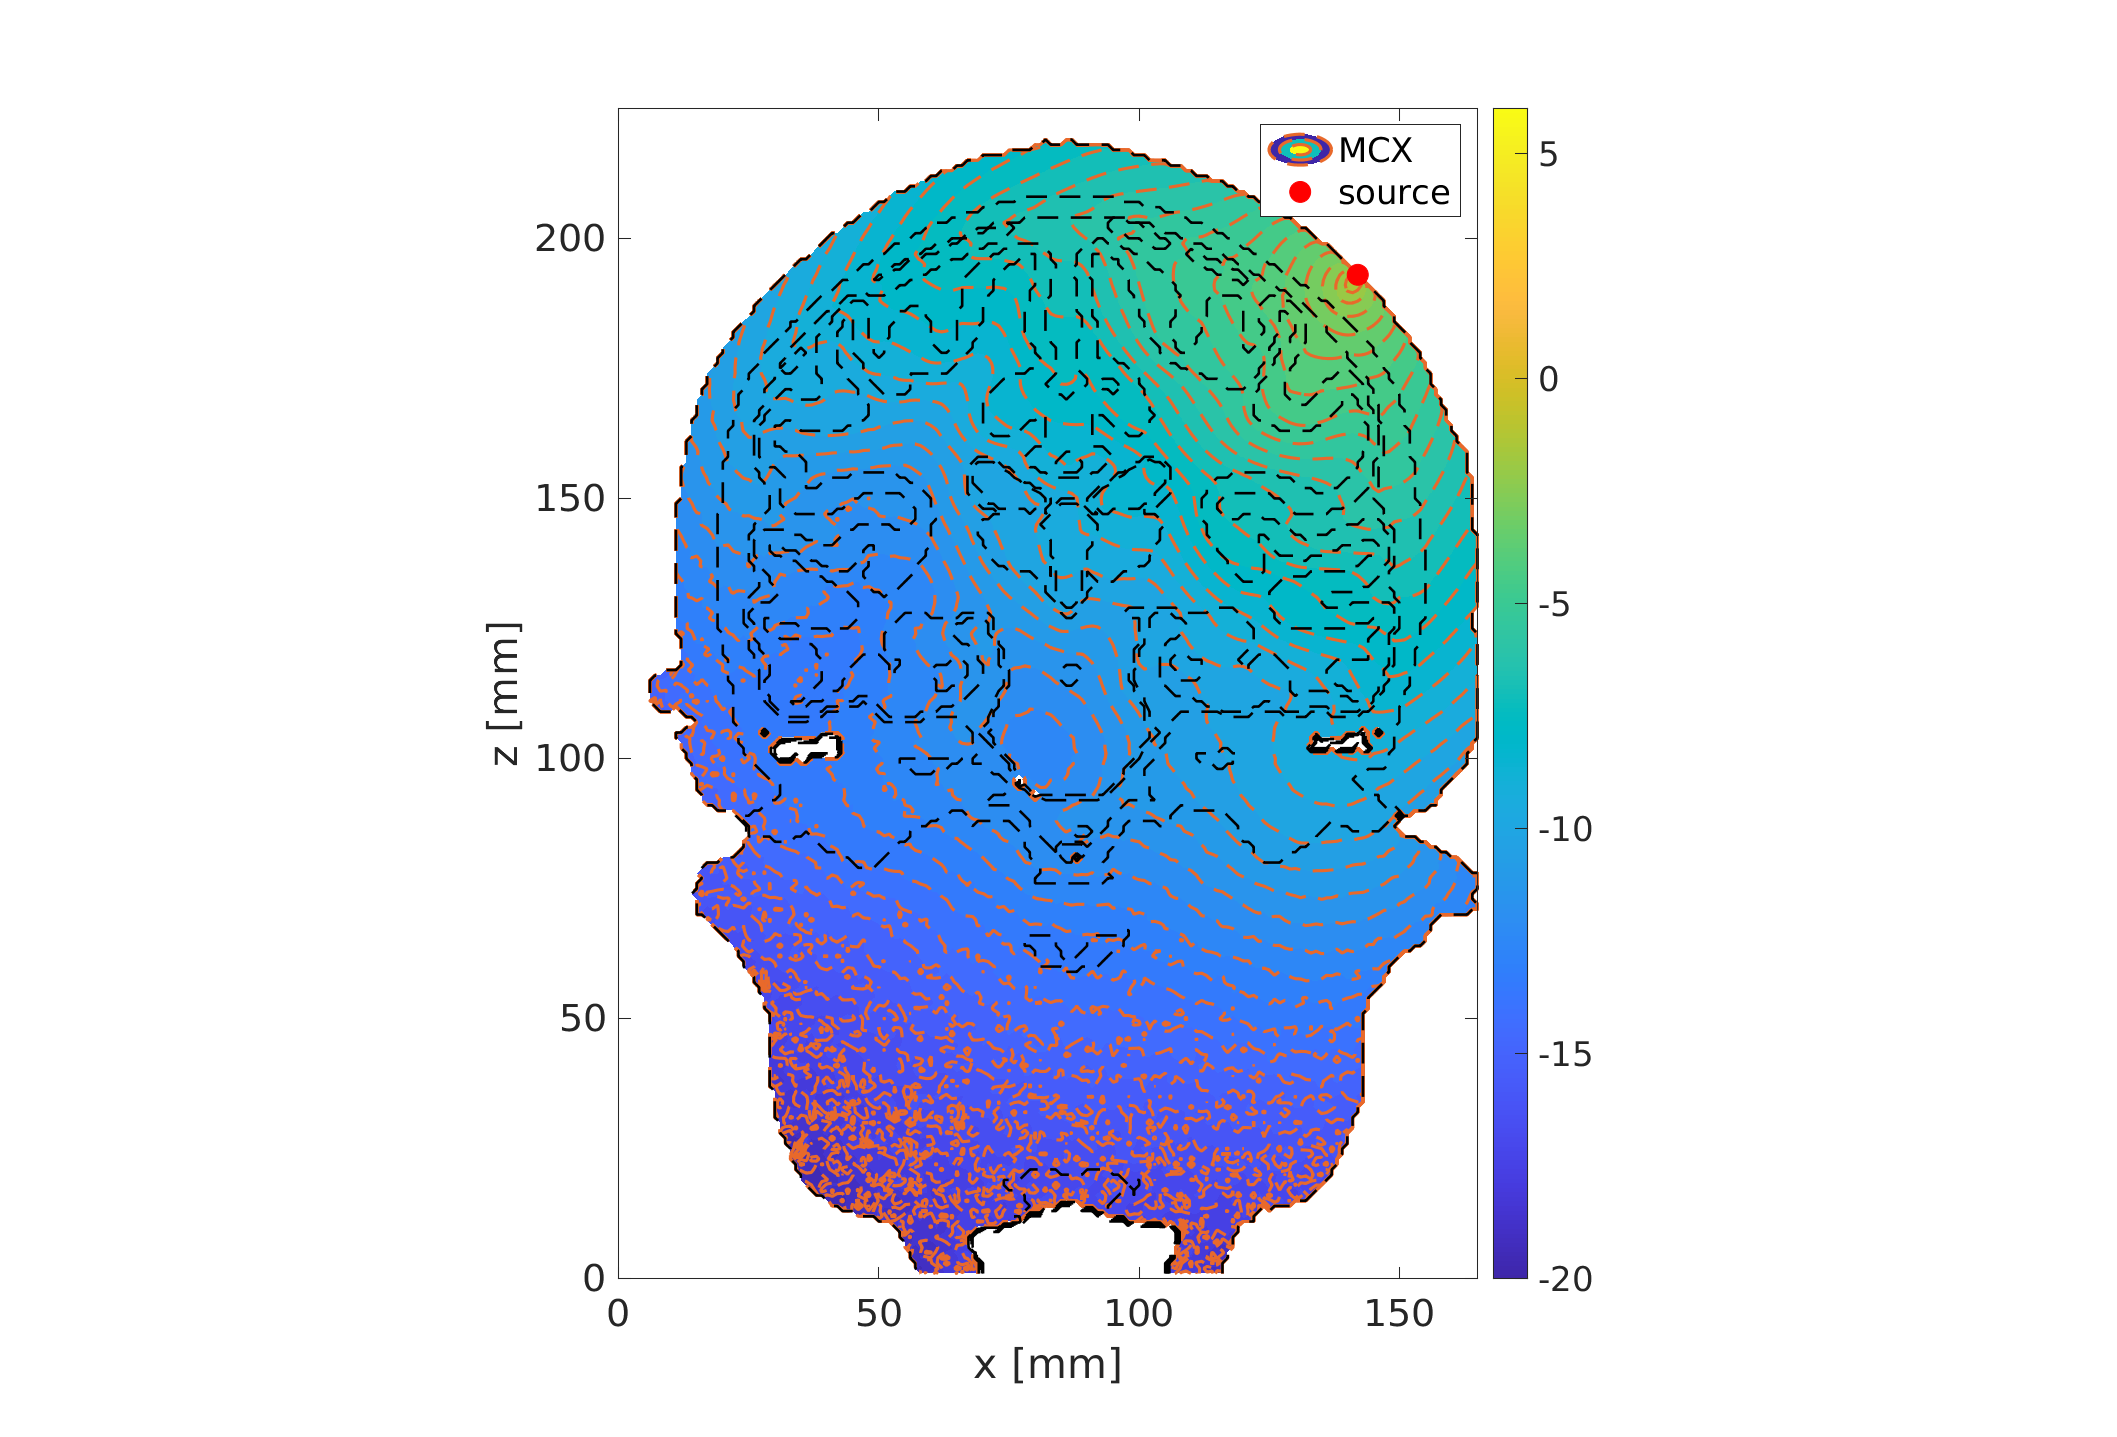
\includegraphics[width=\columnwidth]
    {Figures/Fluence_Distribution_810nm_45deg.png}}
    \caption{\label{fig:810-45} 810 nm 45 Degree Position}
\end{figure}

\begin{figure}[!htb]
    \center{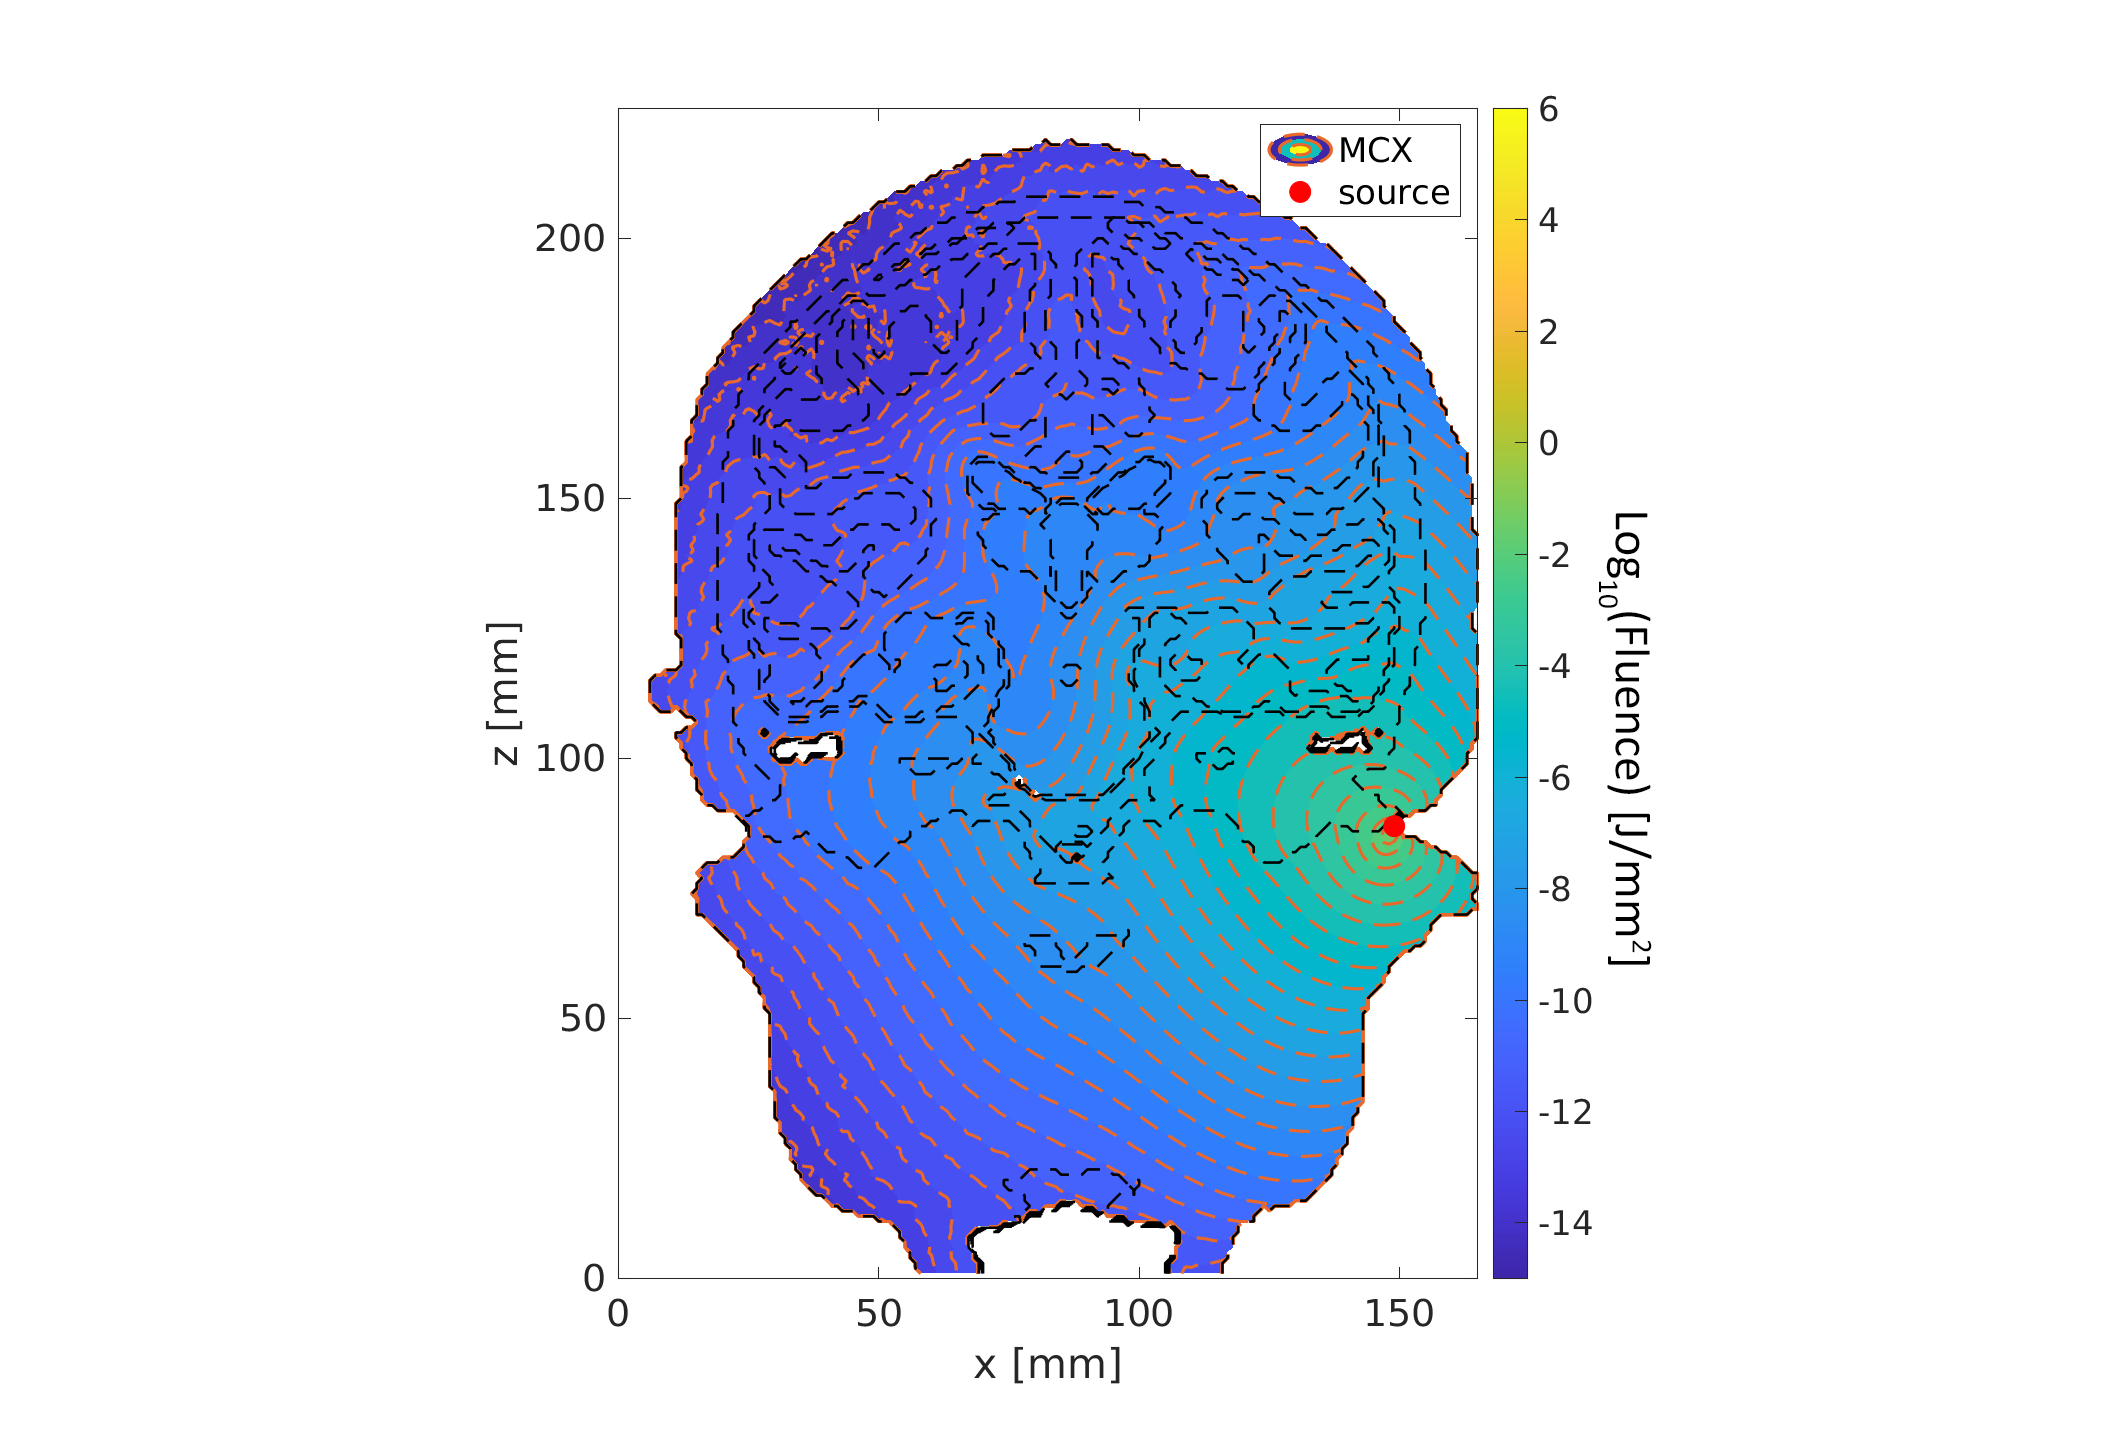
\includegraphics[width=\columnwidth]
    {Figures/Fluence_Distribution_810nm_Cochlear.png}}
    \caption{\label{fig:810-Cochlear} 810 nm Cochlear Position}
\end{figure}

\begin{figure}[!htb]
    \center{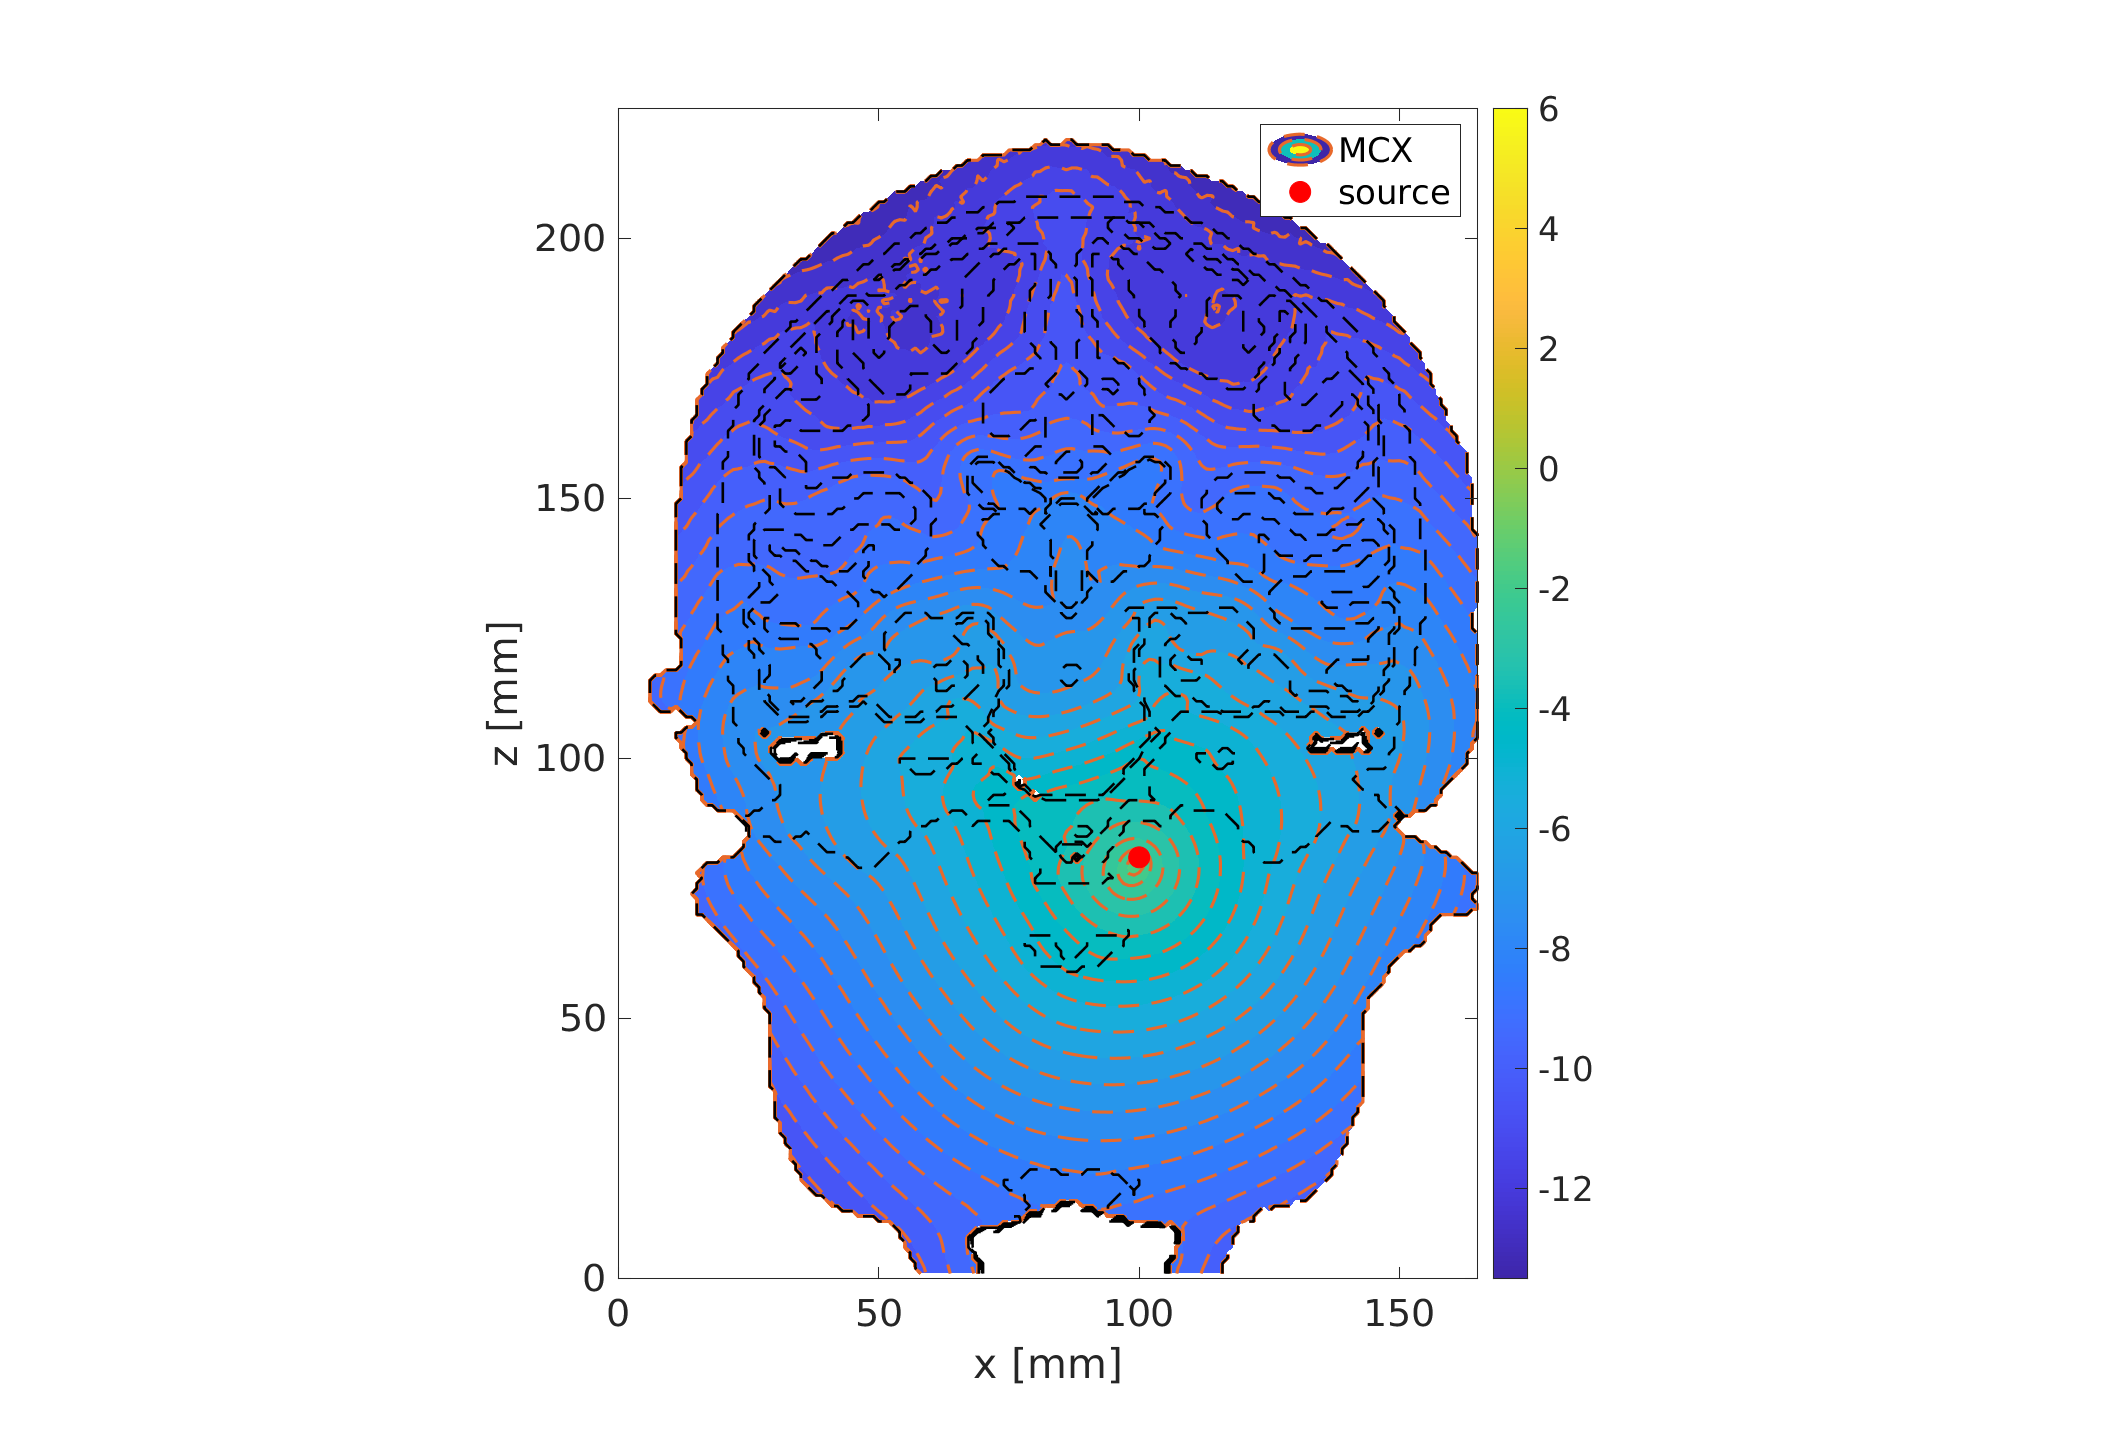
\includegraphics[width=\columnwidth]
    {Figures/Fluence_Distribution_810nm_Intranasal.png}}
    \caption{\label{fig:810-Intra} 810 nm Intranasal Position}
\end{figure}

\begin{figure}[!htb]
    \center{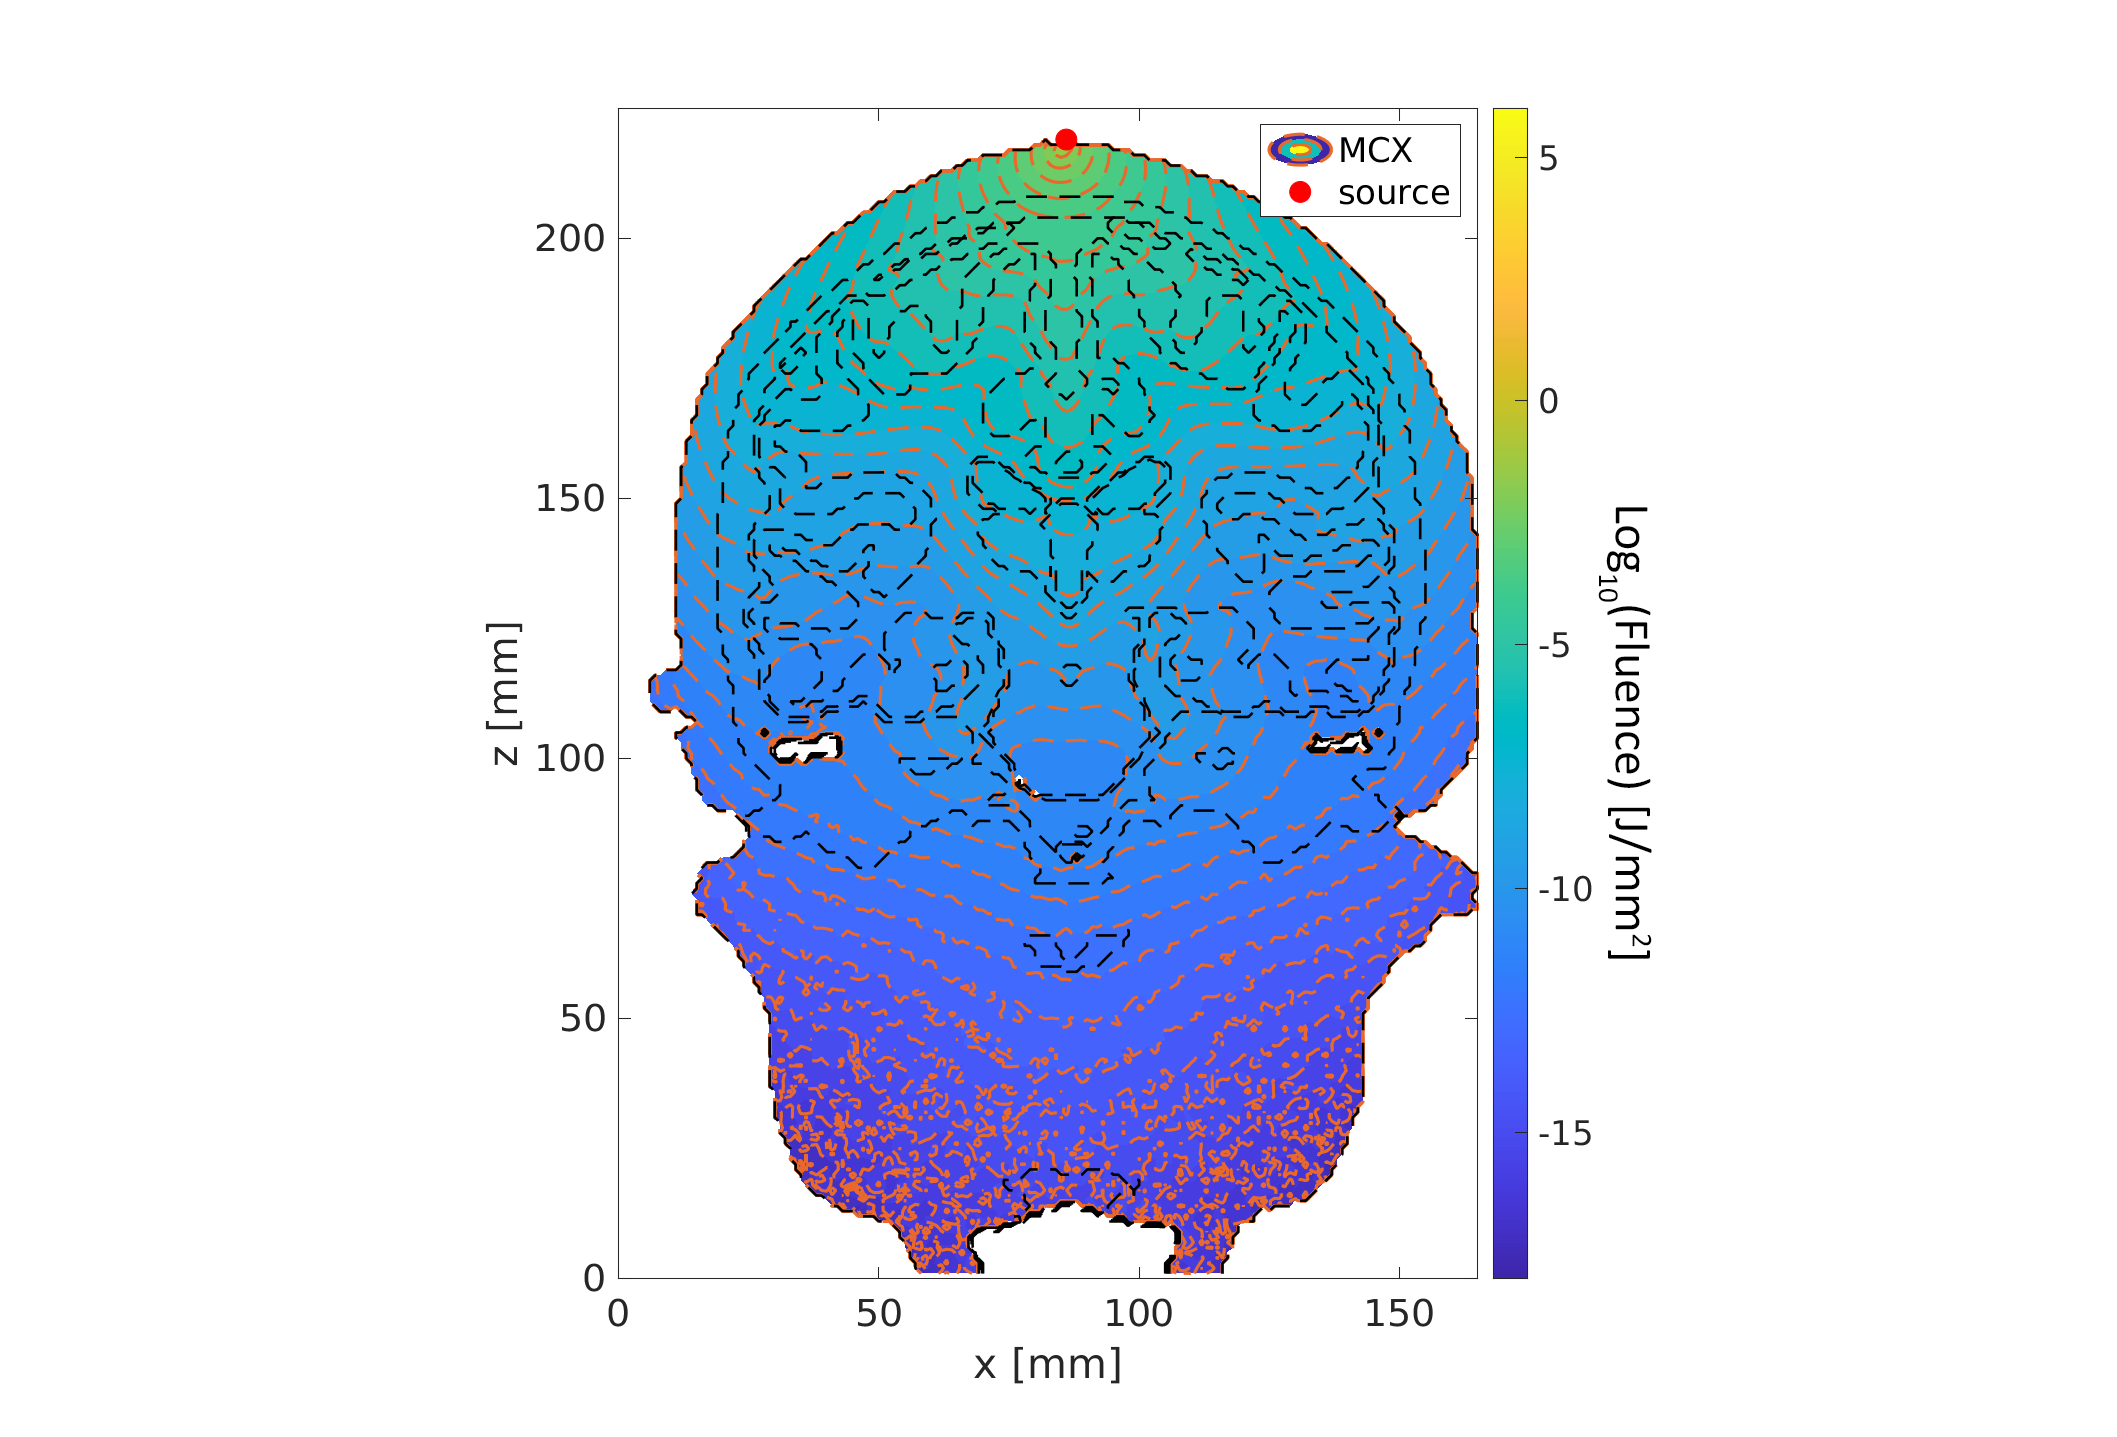
\includegraphics[width=\columnwidth]
    {Figures/Fluence_Distribution_980nm_CZ.png}}
    \caption{\label{fig:980-CZ} 980 nm CZ Position}
\end{figure}

\begin{figure}[!htb]
    \center{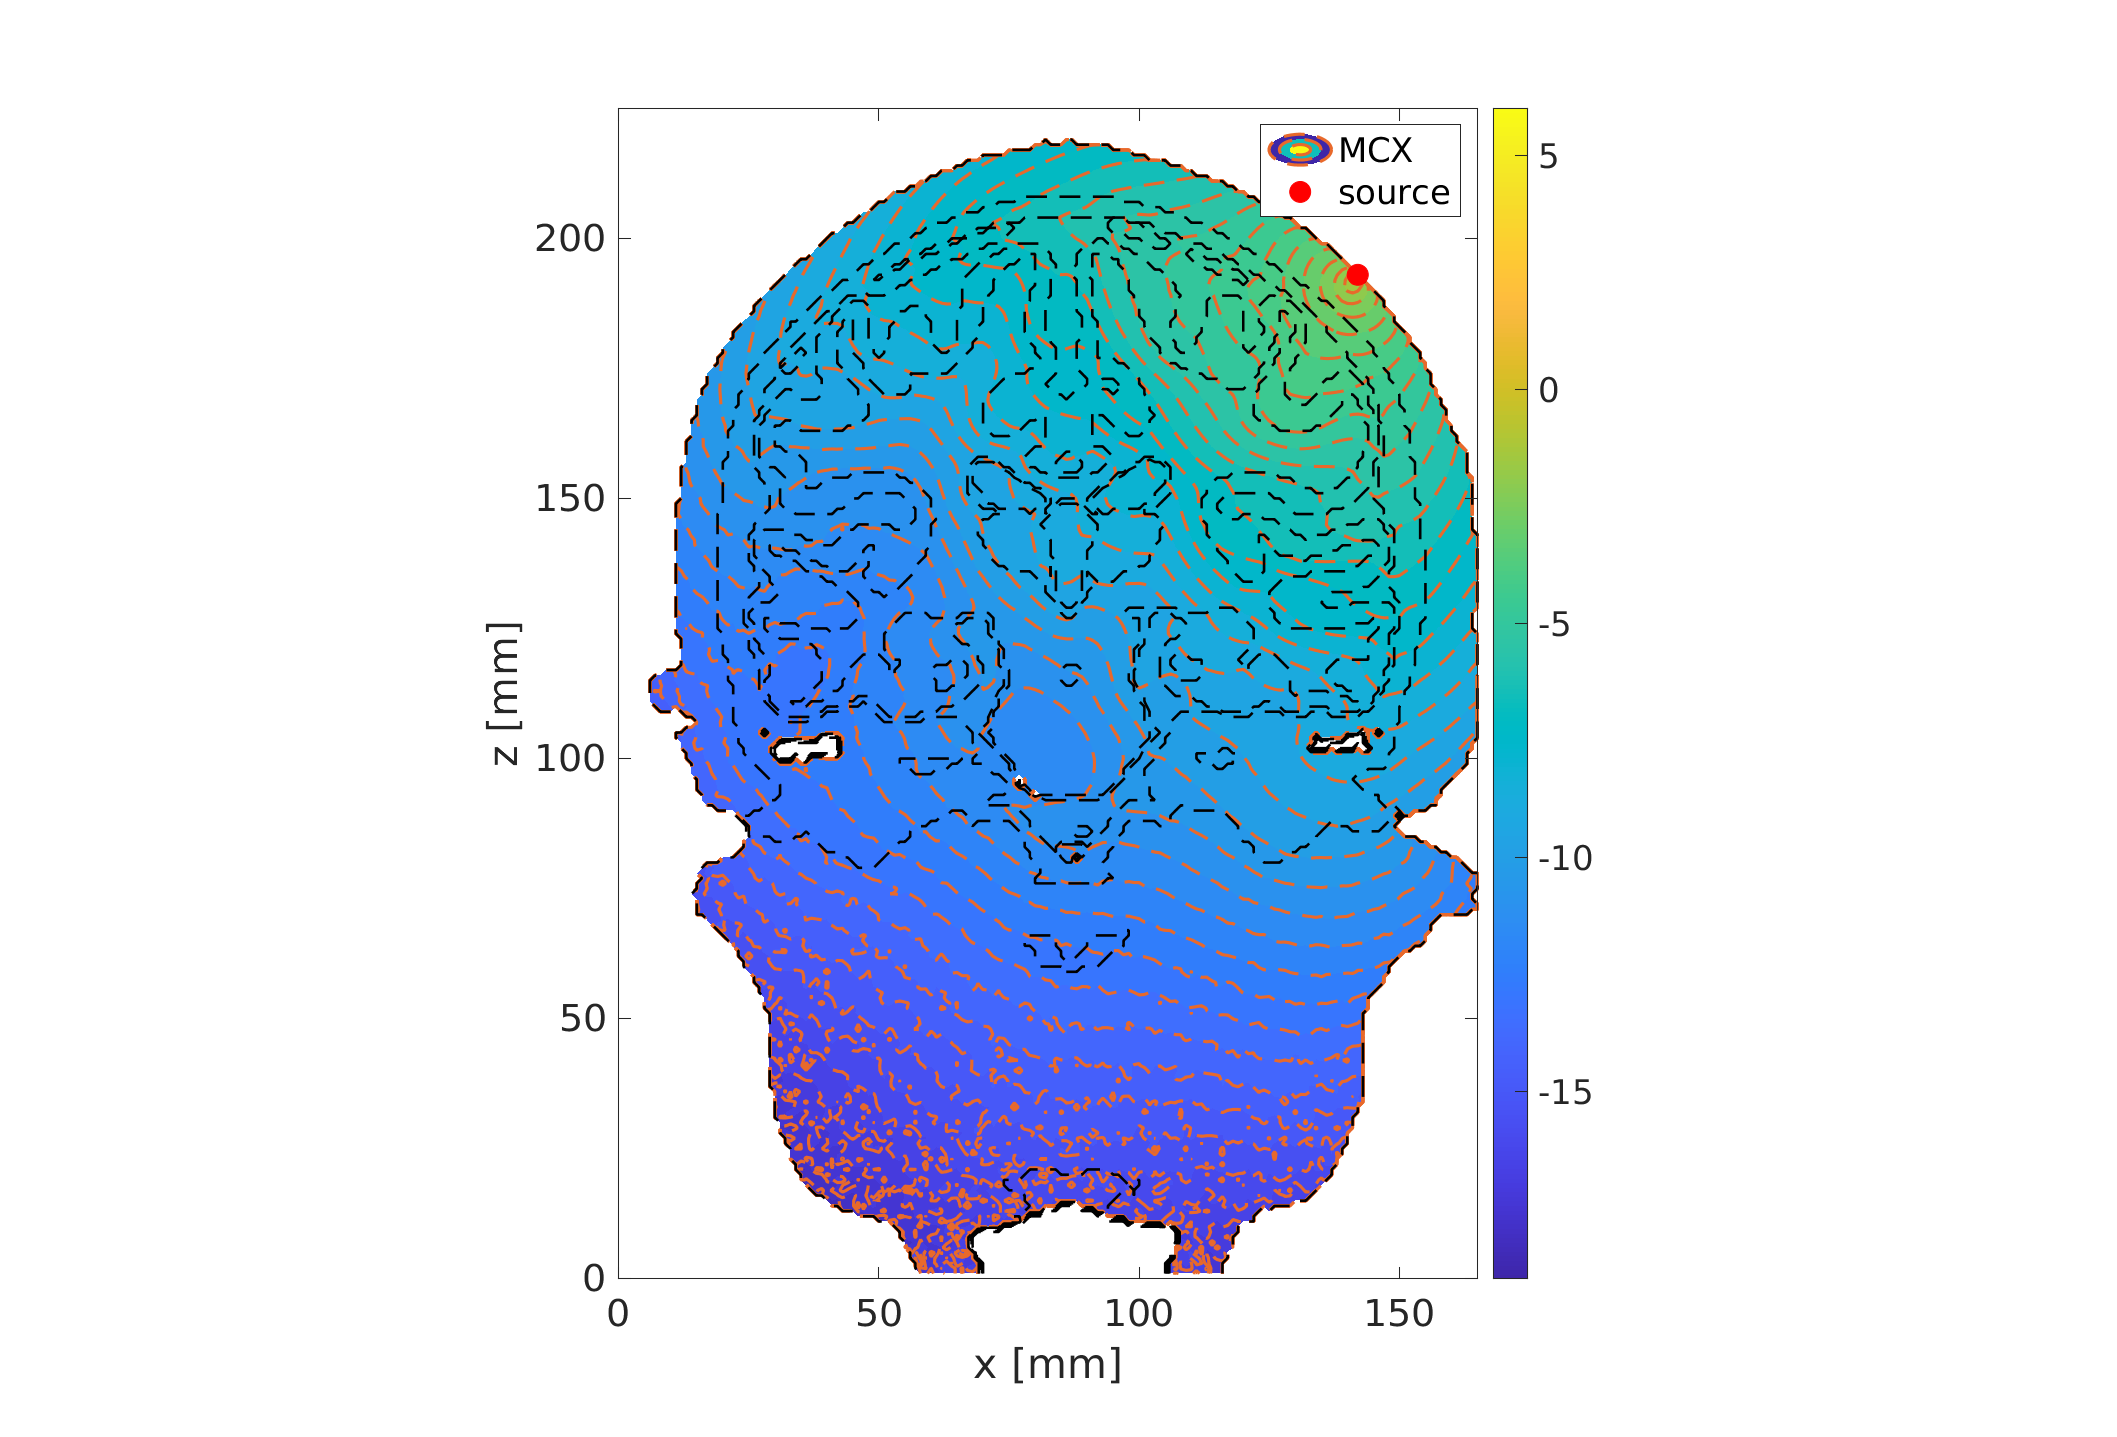
\includegraphics[width=\columnwidth]
    {Figures/Fluence_Distribution_980nm_45deg.png}}
    \caption{\label{fig:980-45} 980 nm 45 Degree Position}
\end{figure}

\begin{figure}[!htb]
    \center{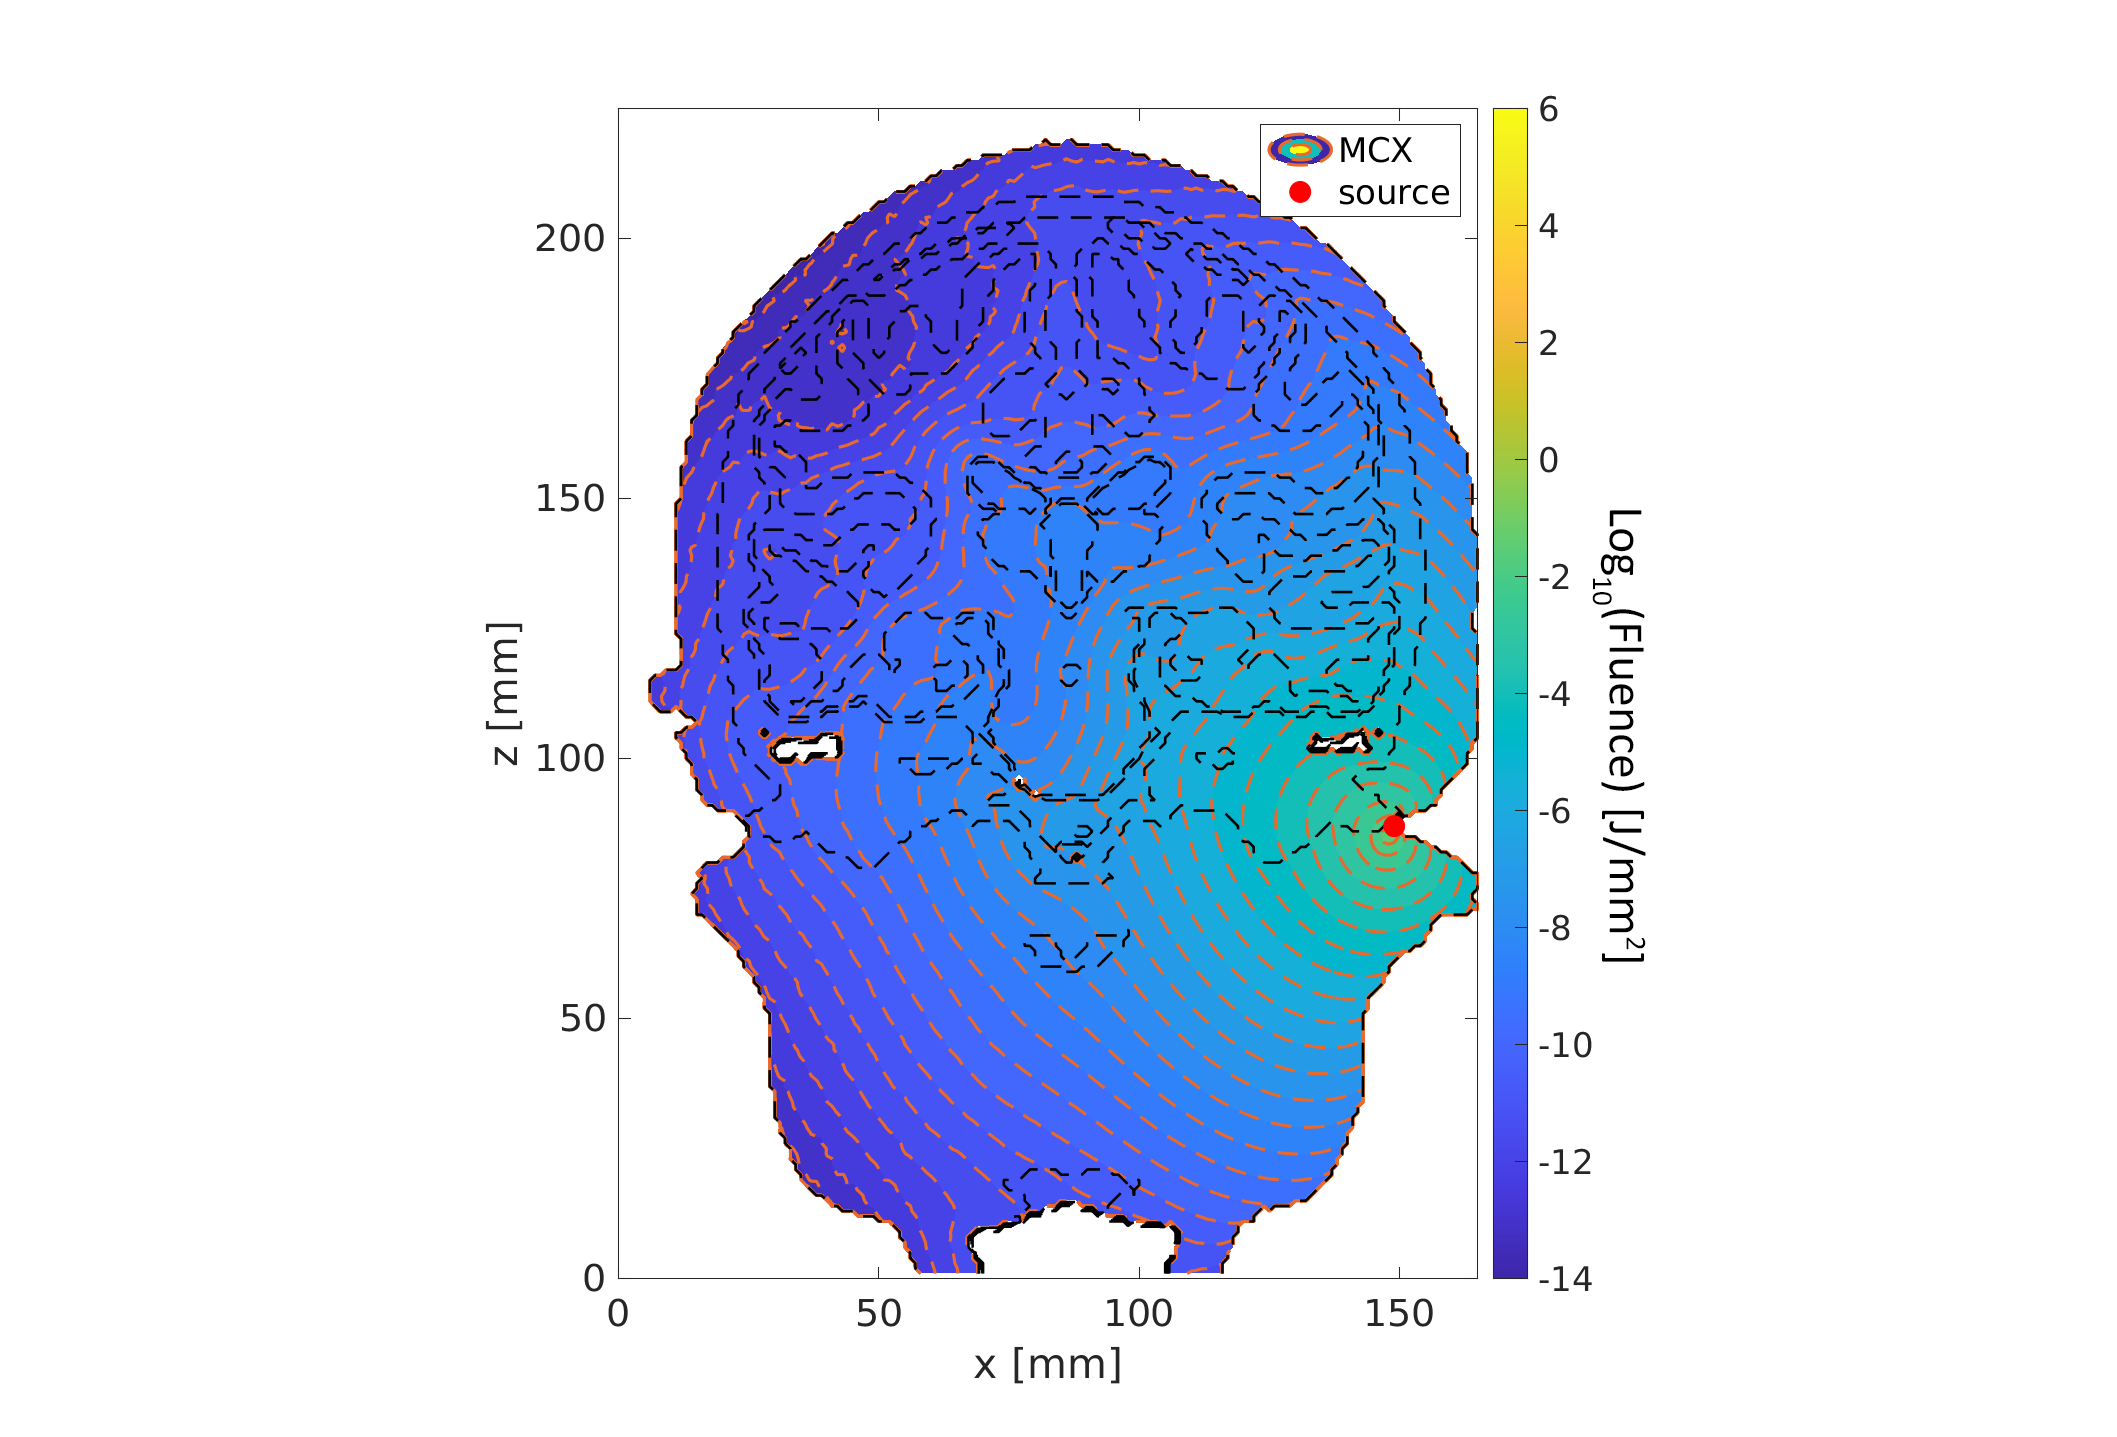
\includegraphics[width=\columnwidth]
    {Figures/Fluence_Distribution_980nm_Cochlear.png}}
    \caption{\label{fig:980-Cochlear} 980 nm Cochlear Position}
\end{figure}

\begin{figure}[!htb]
    \center{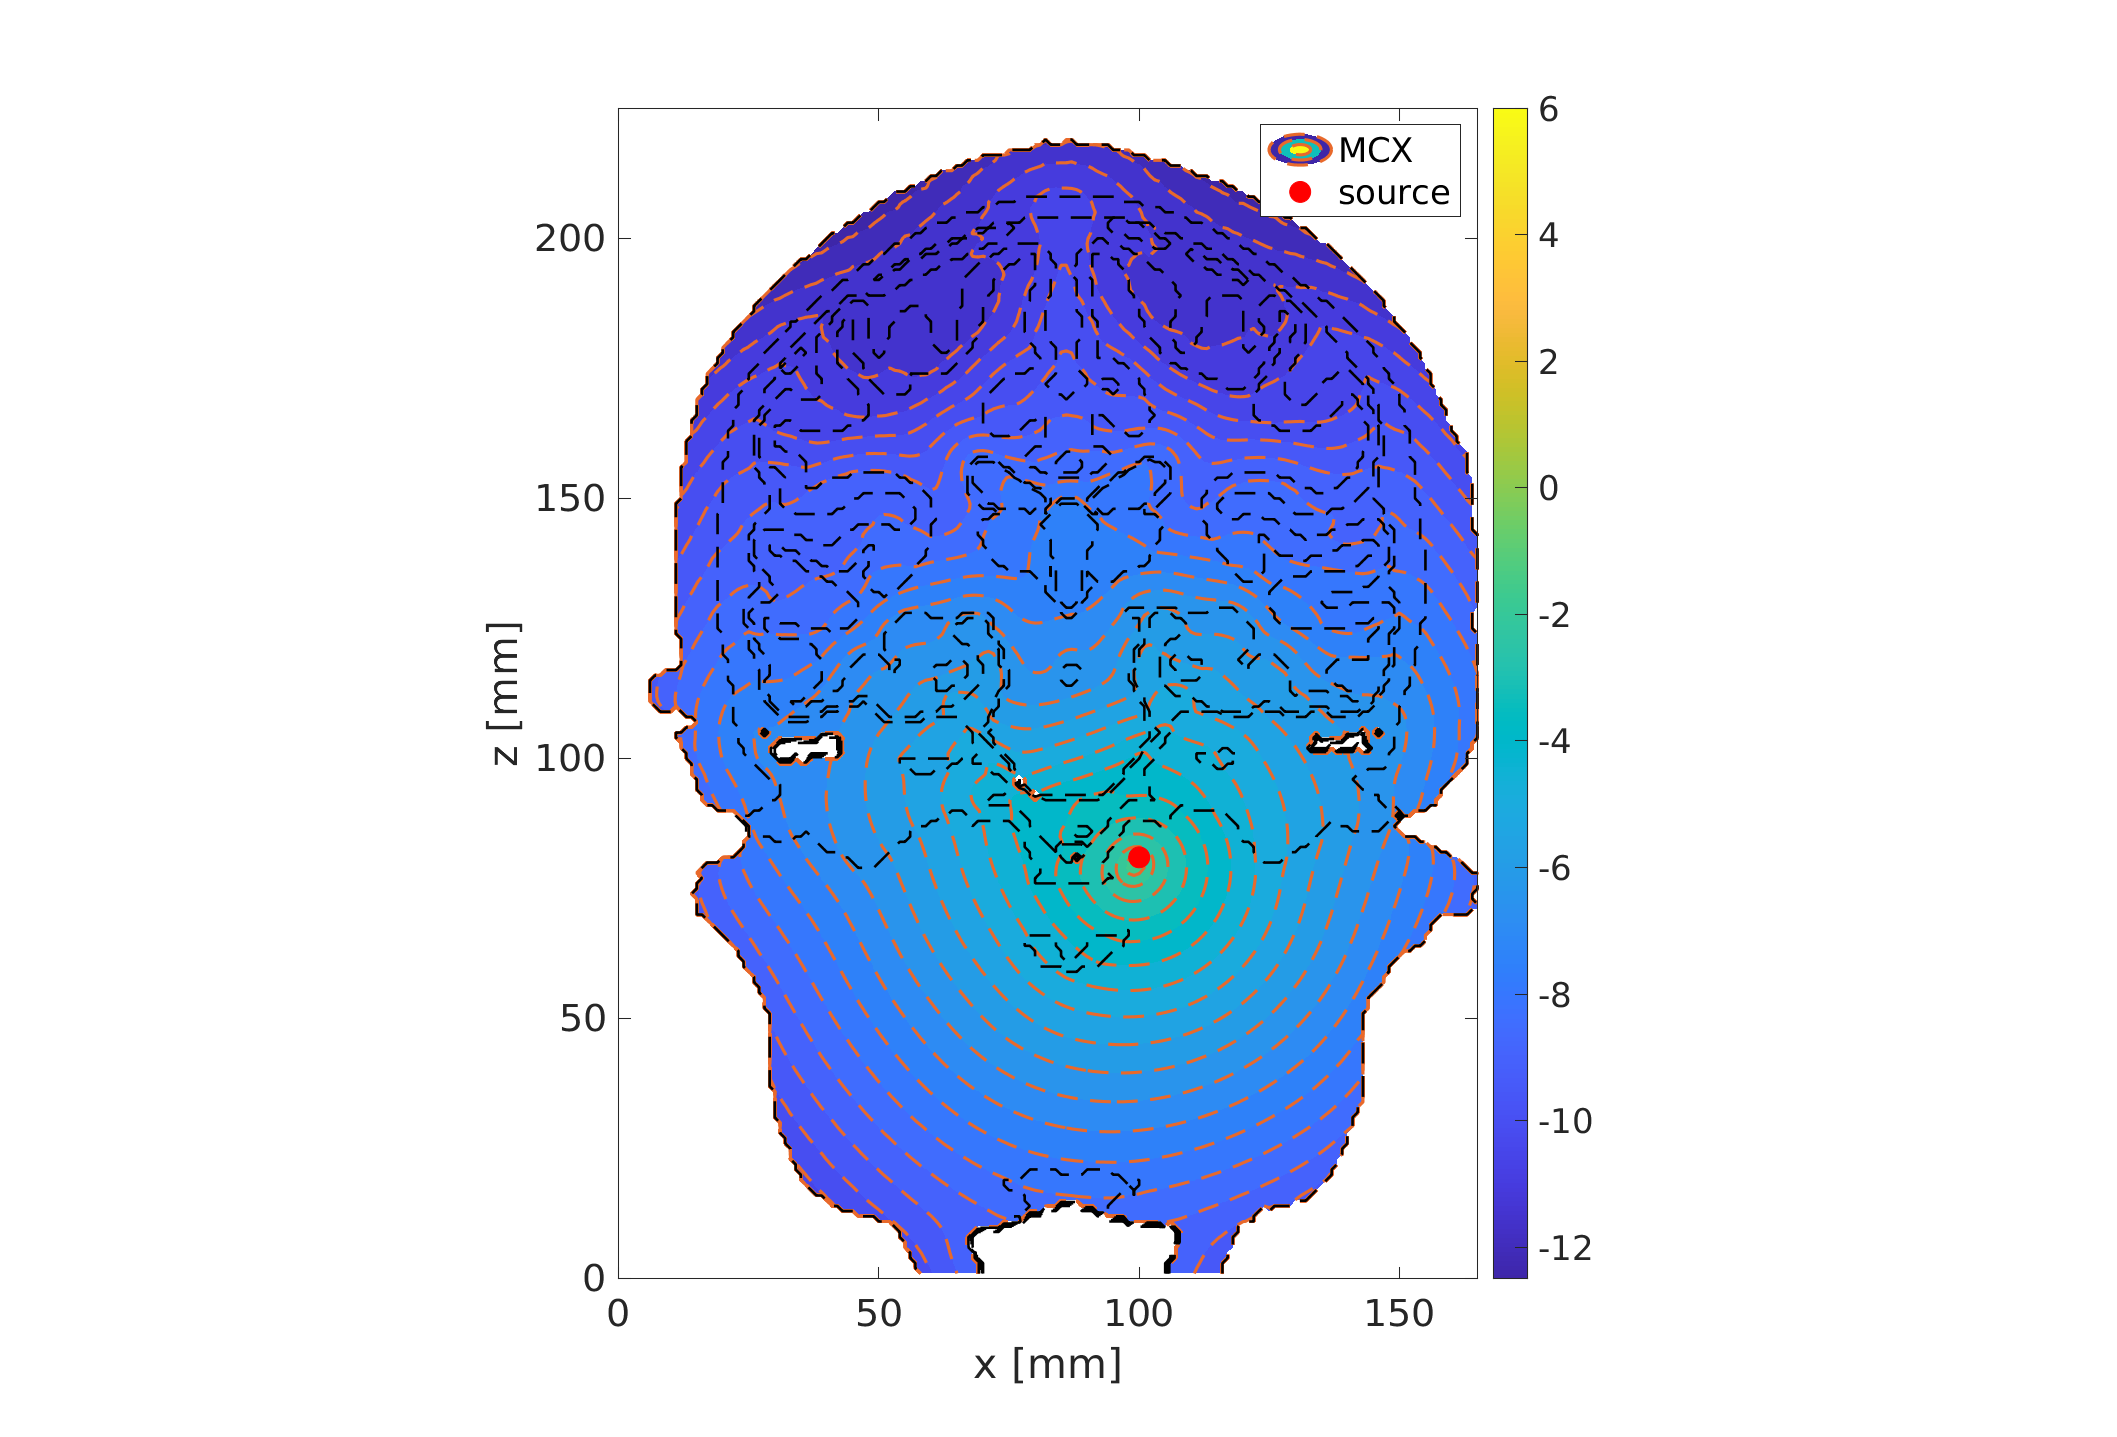
\includegraphics[width=\columnwidth]
    {Figures/Fluence_Distribution_980nm_Intranasal.png}}
    \caption{\label{fig:980-Intra} 980 nm Intranasal Position}
\end{figure}

\begin{figure}[!htb]
    \center{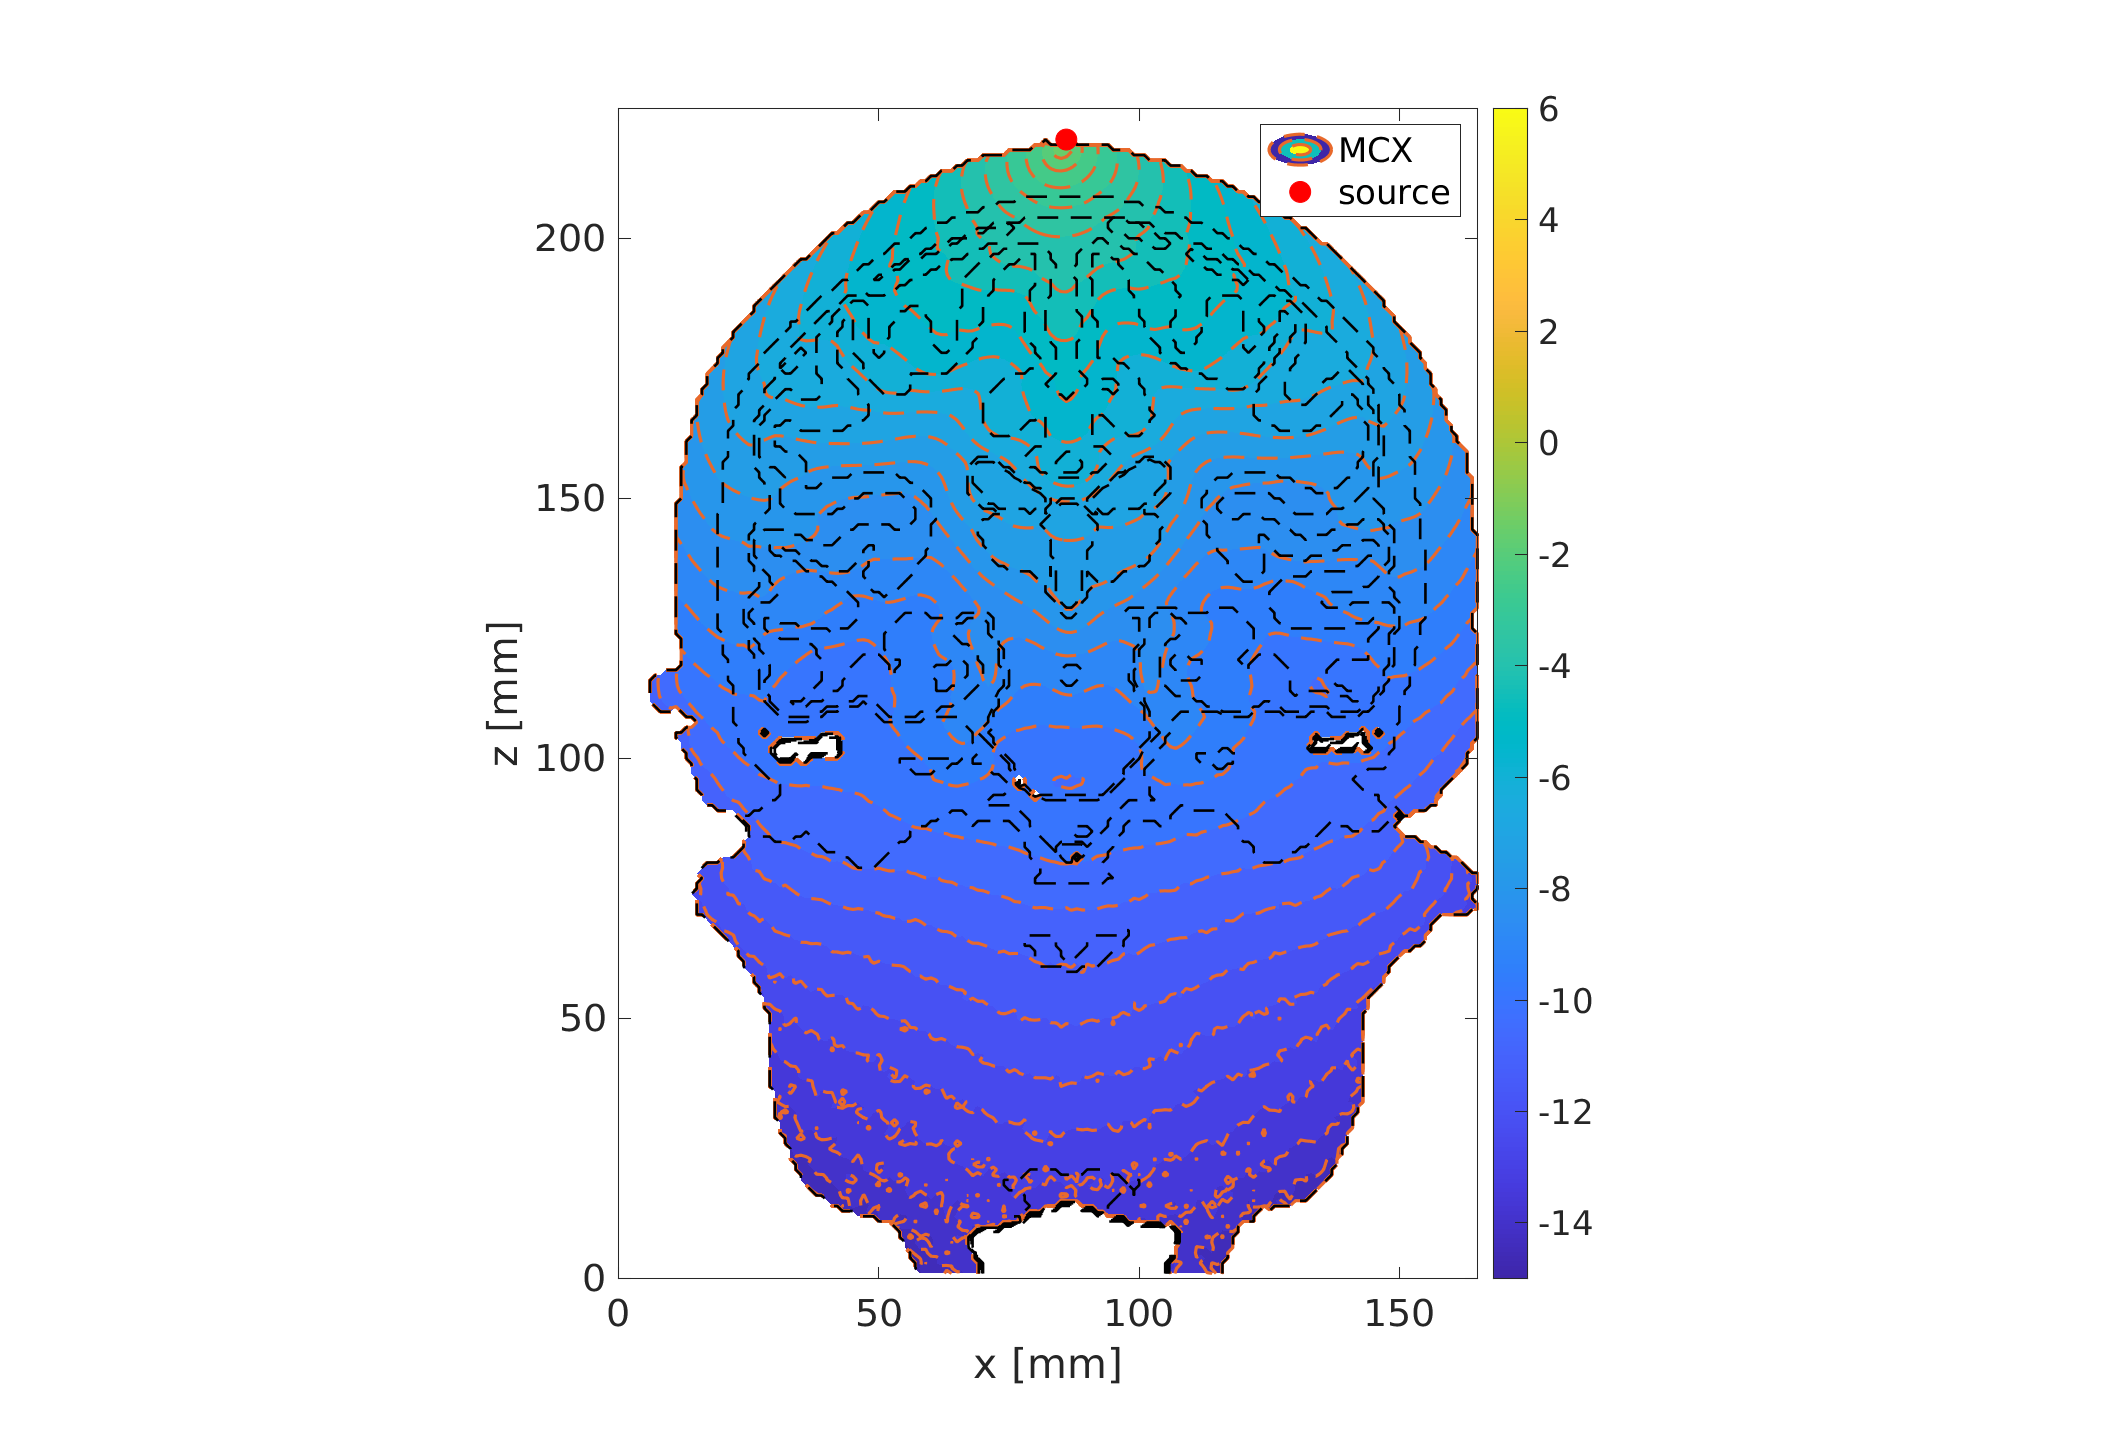
\includegraphics[width=\columnwidth]
    {Figures/Fluence_Distribution_1064nm_CZ.png}}
    \caption{\label{fig:1064-CZ} 1064 nm CZ Position}
\end{figure}

\begin{figure}[!htb]
    \center{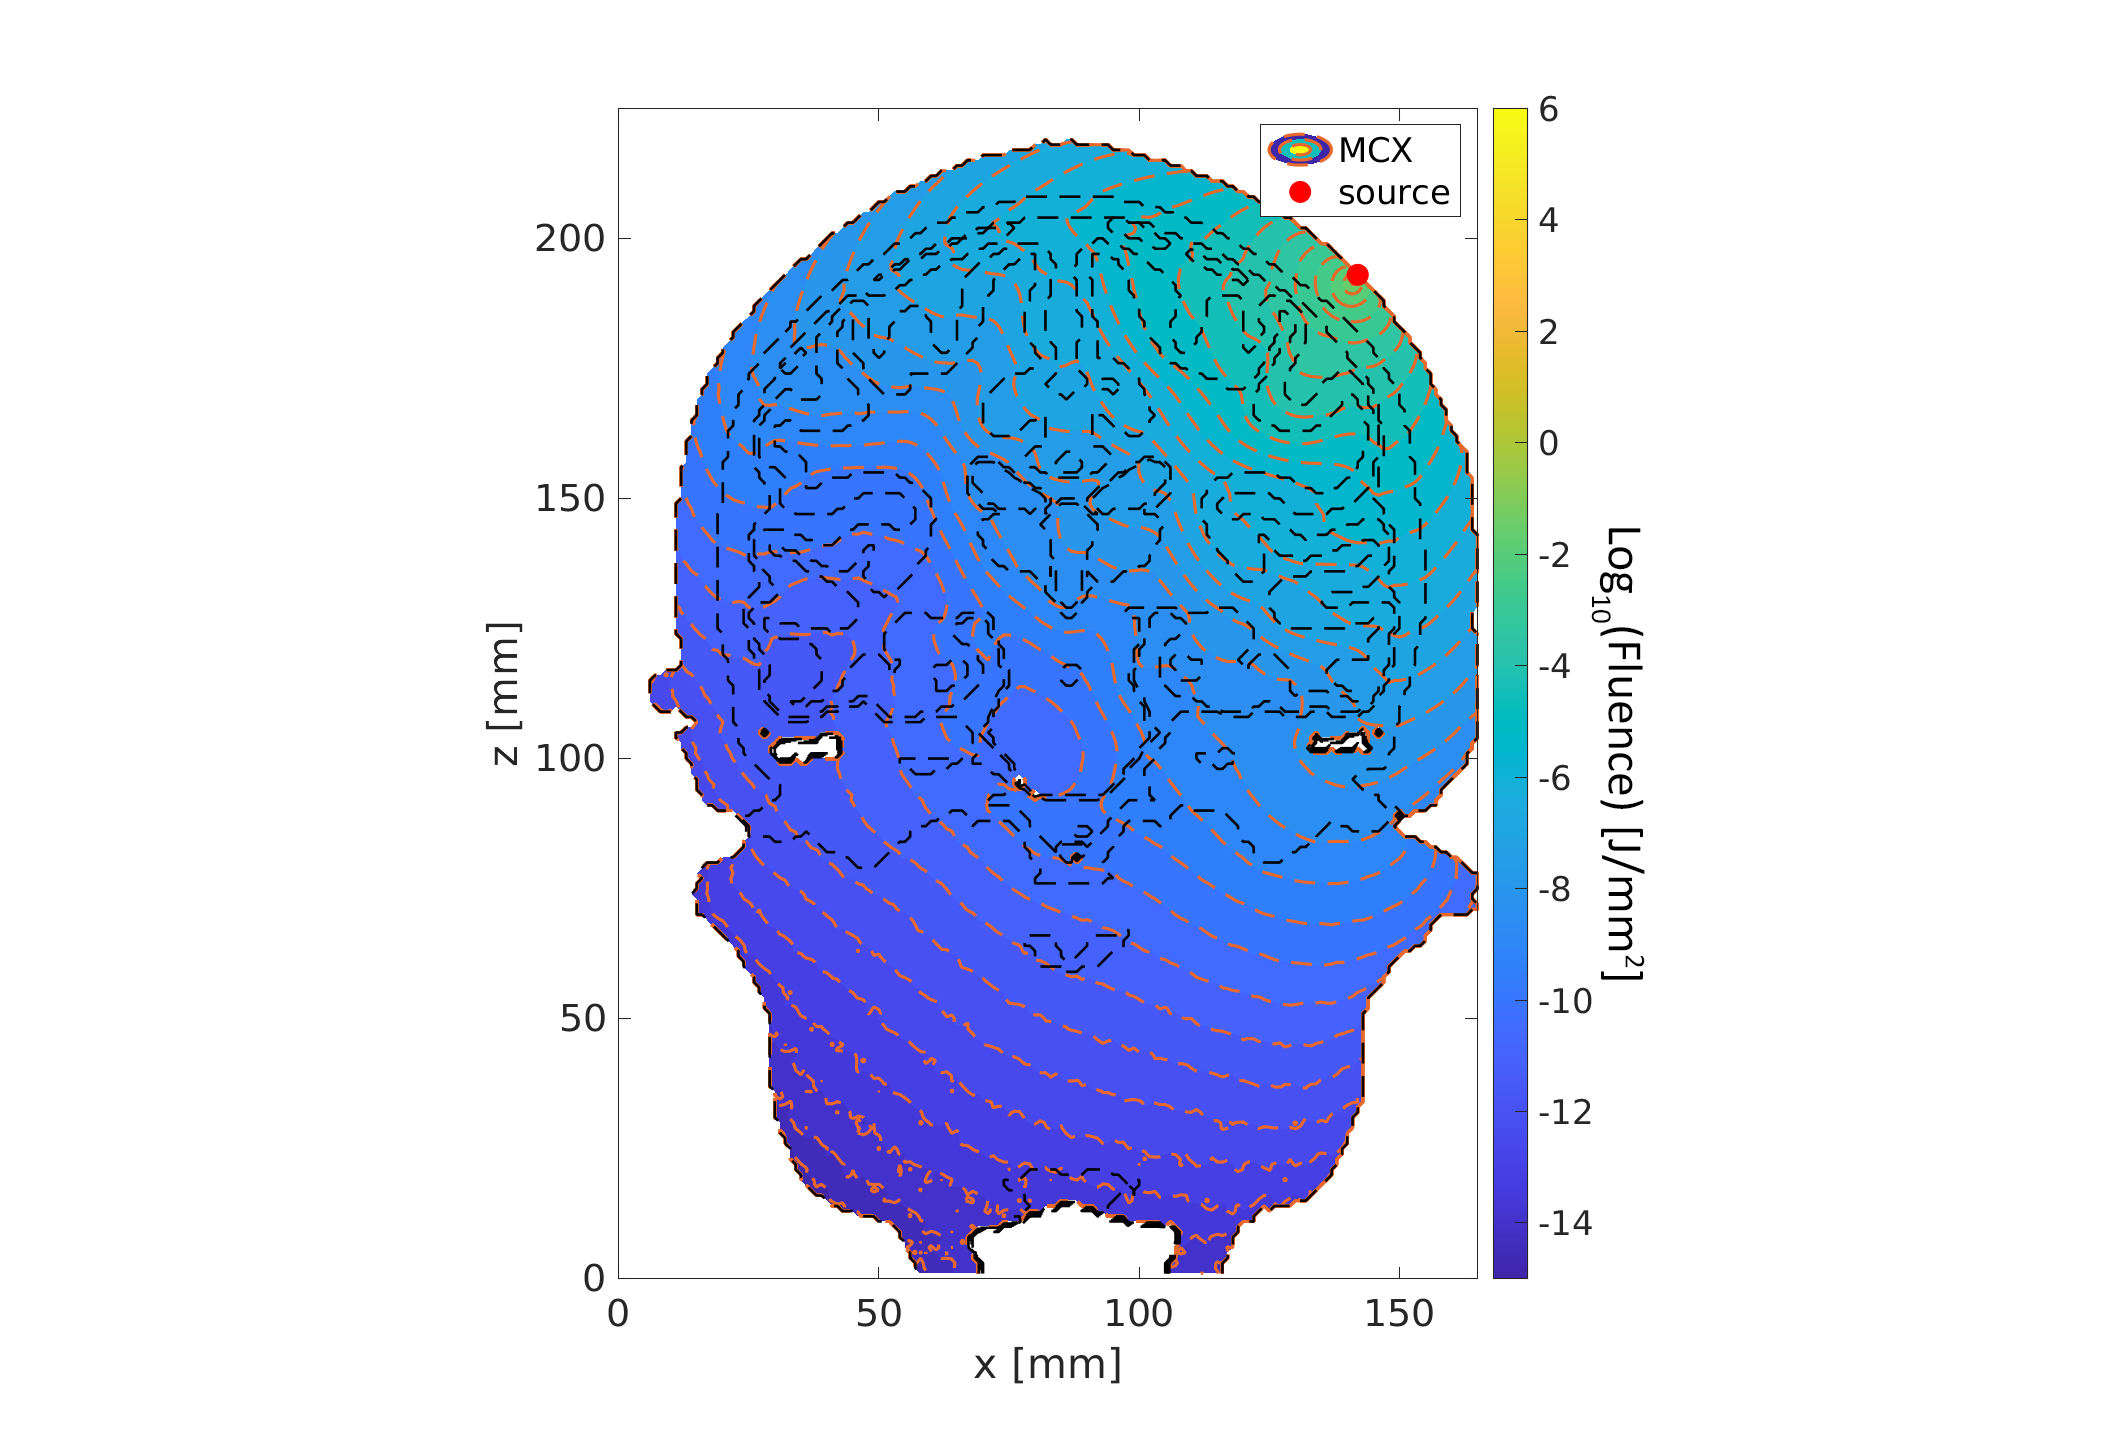
\includegraphics[width=\columnwidth]
    {Figures/Fluence_Distribution_1064nm_45deg.png}}
    \caption{\label{fig:1064-45} 1064 nm 45 Degree Position}
\end{figure}

\begin{figure}[!htb]
    \center{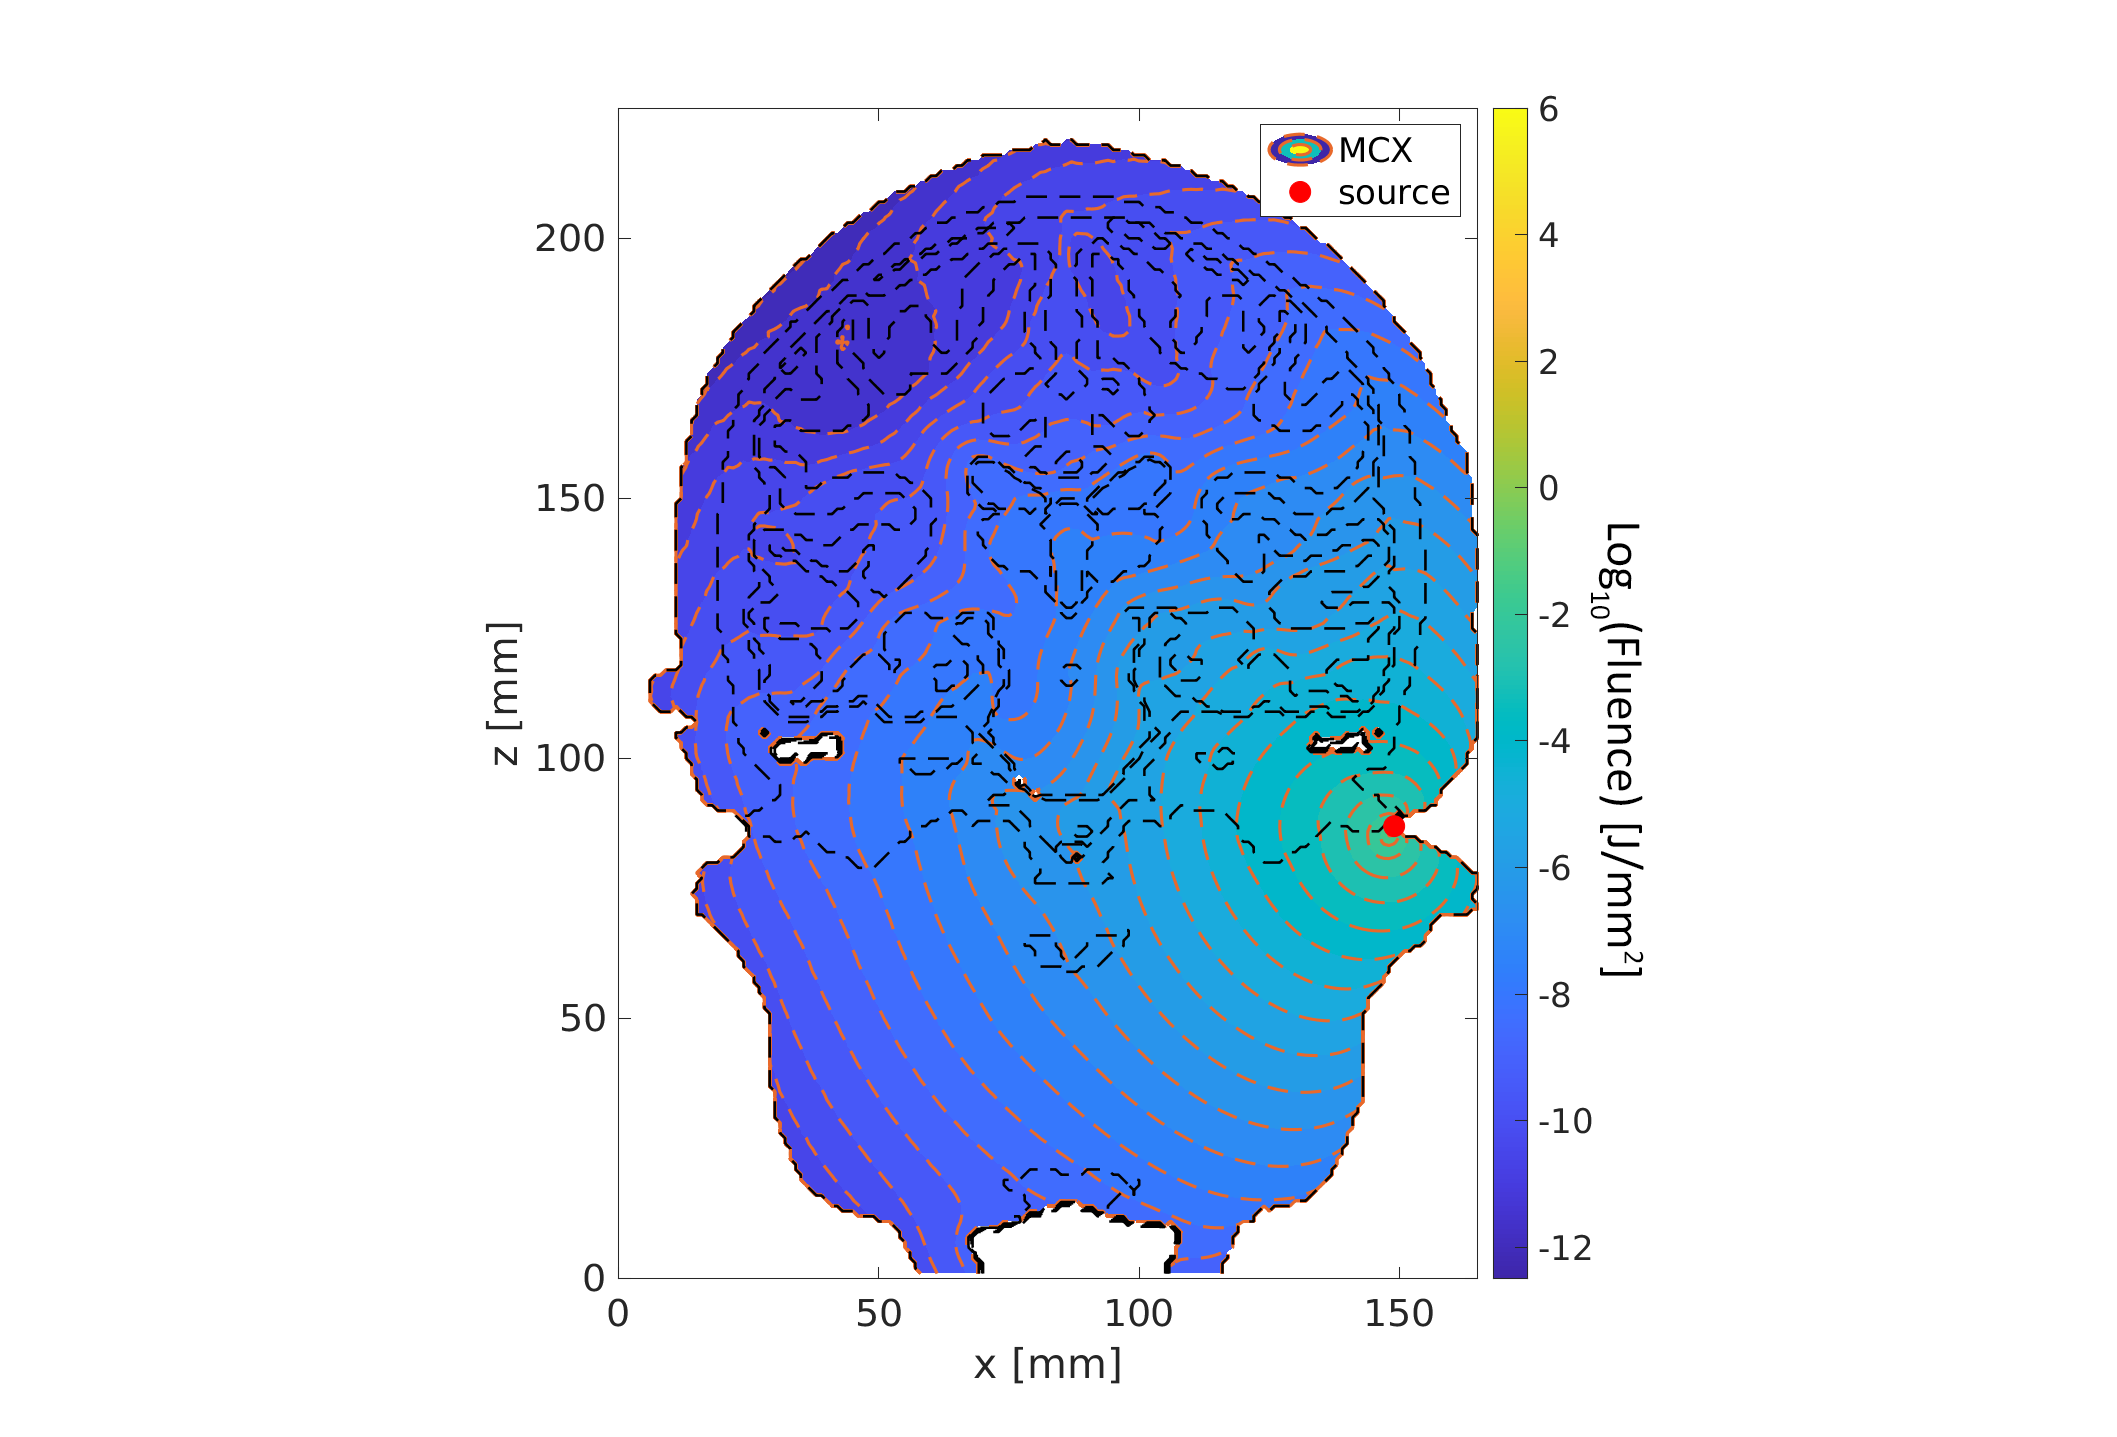
\includegraphics[width=\columnwidth]
    {Figures/Fluence_Distribution_1064nm_Cochlear.png}}
    \caption{\label{fig:1064-Cochlear} 1064 nm Cochlear Position}
\end{figure}

\begin{figure}[!htb]
    \center{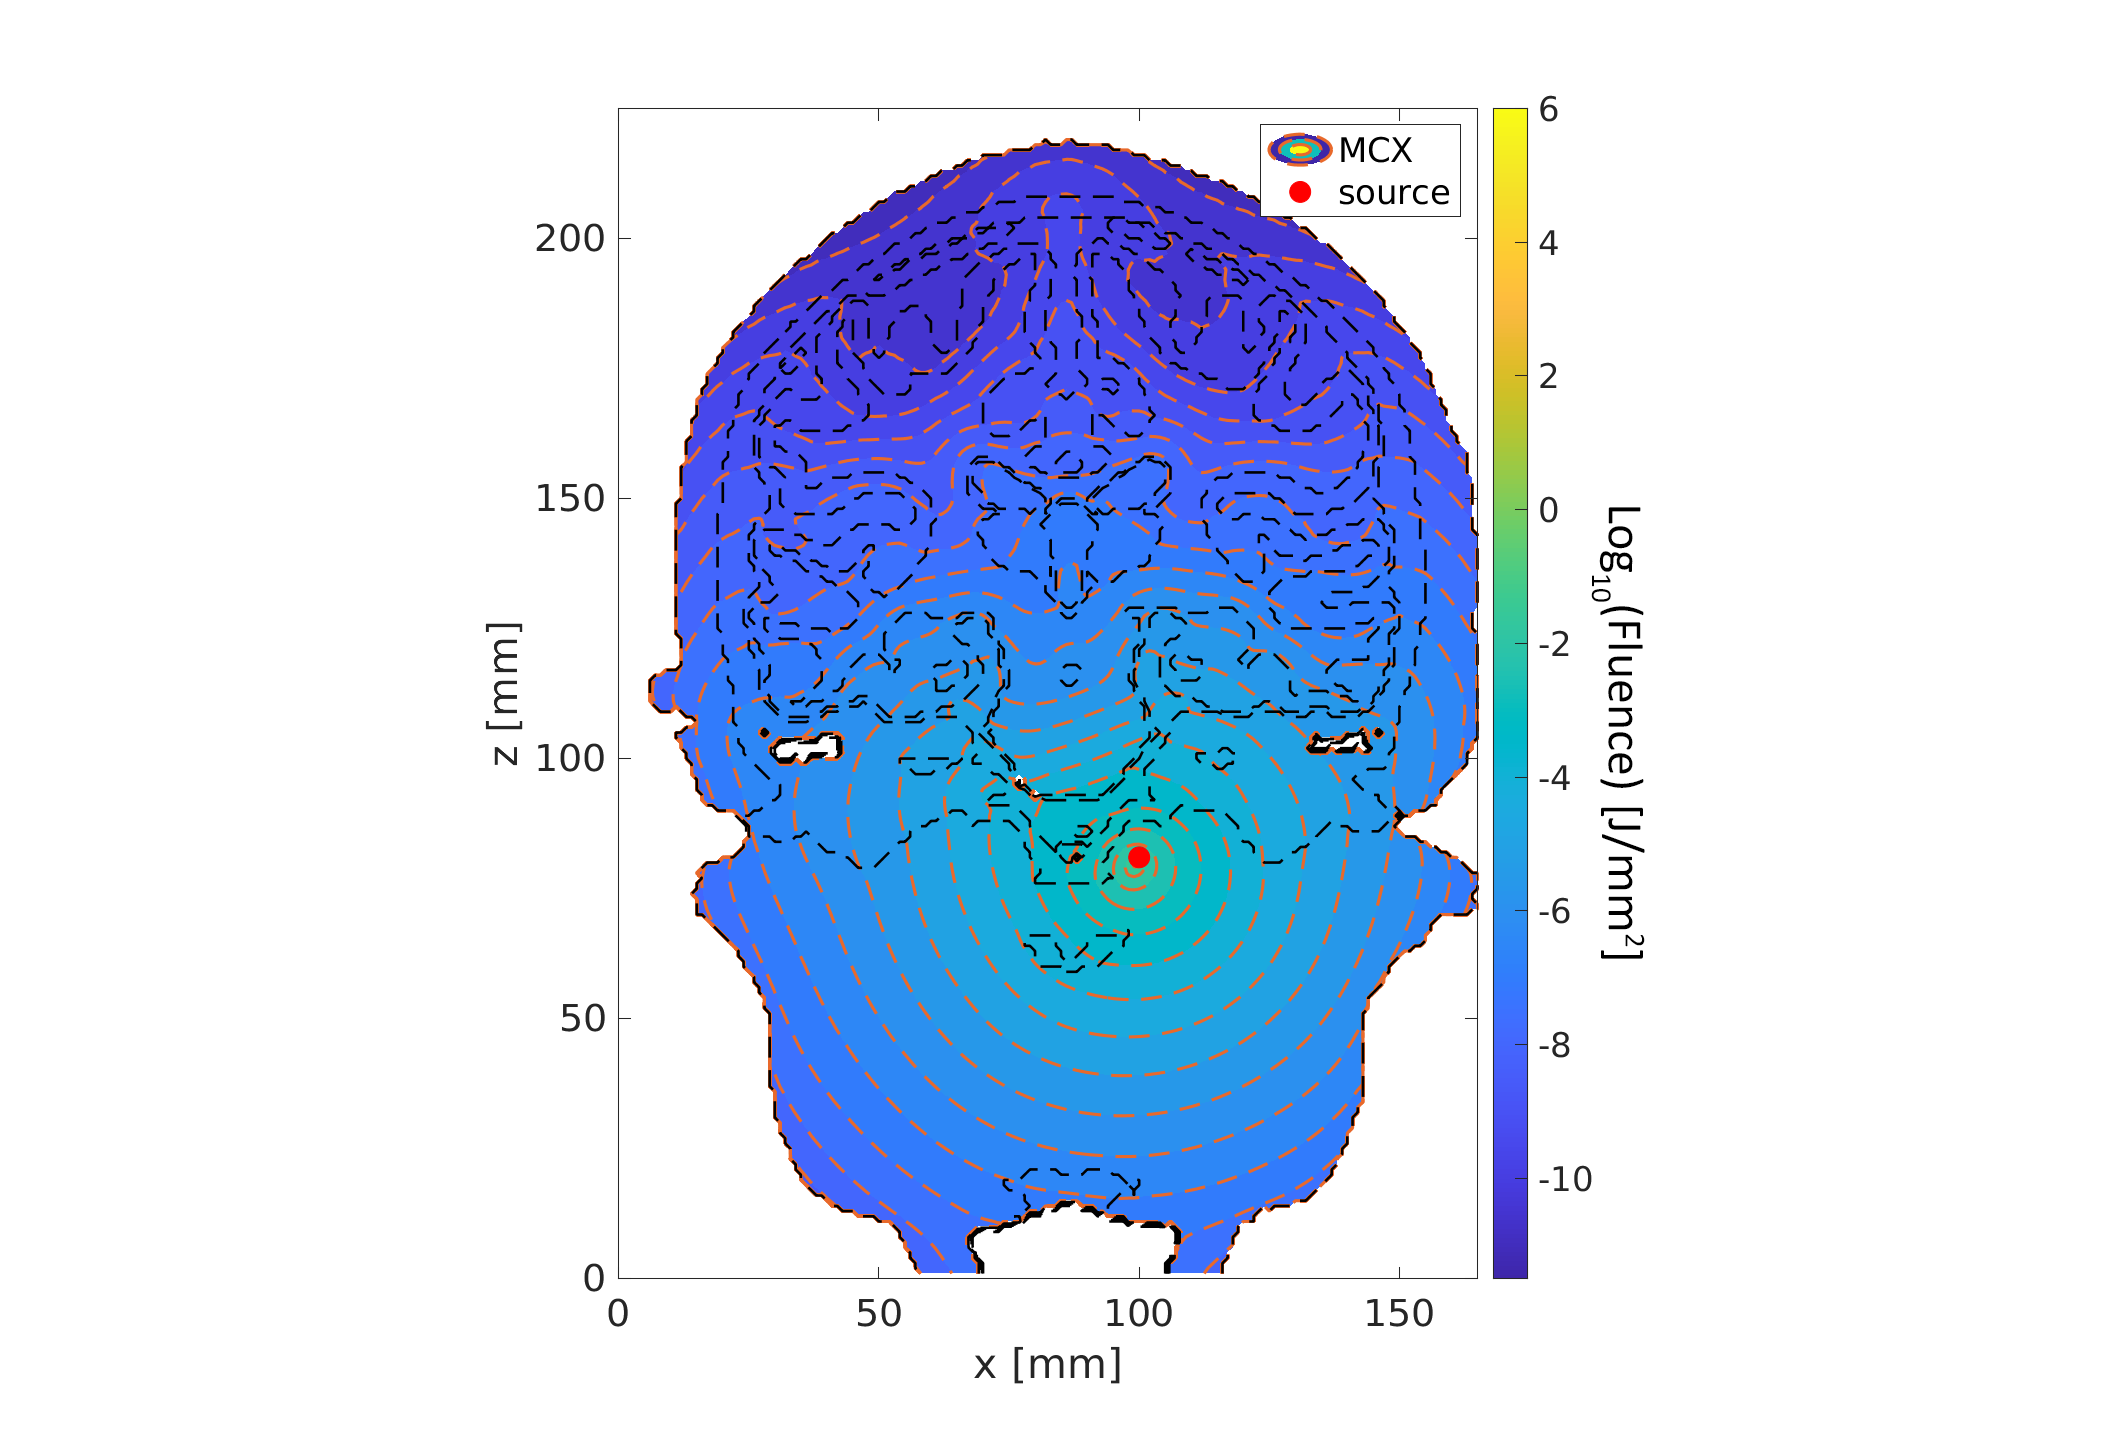
\includegraphics[width=\columnwidth]
    {Figures/Fluence_Distribution_1064nm_Intranasal.png}}
    \caption{\label{fig:1064-Intra} 1064 nm Intranasal Position}
\end{figure}

\begin{figure}[!htb]
    \center{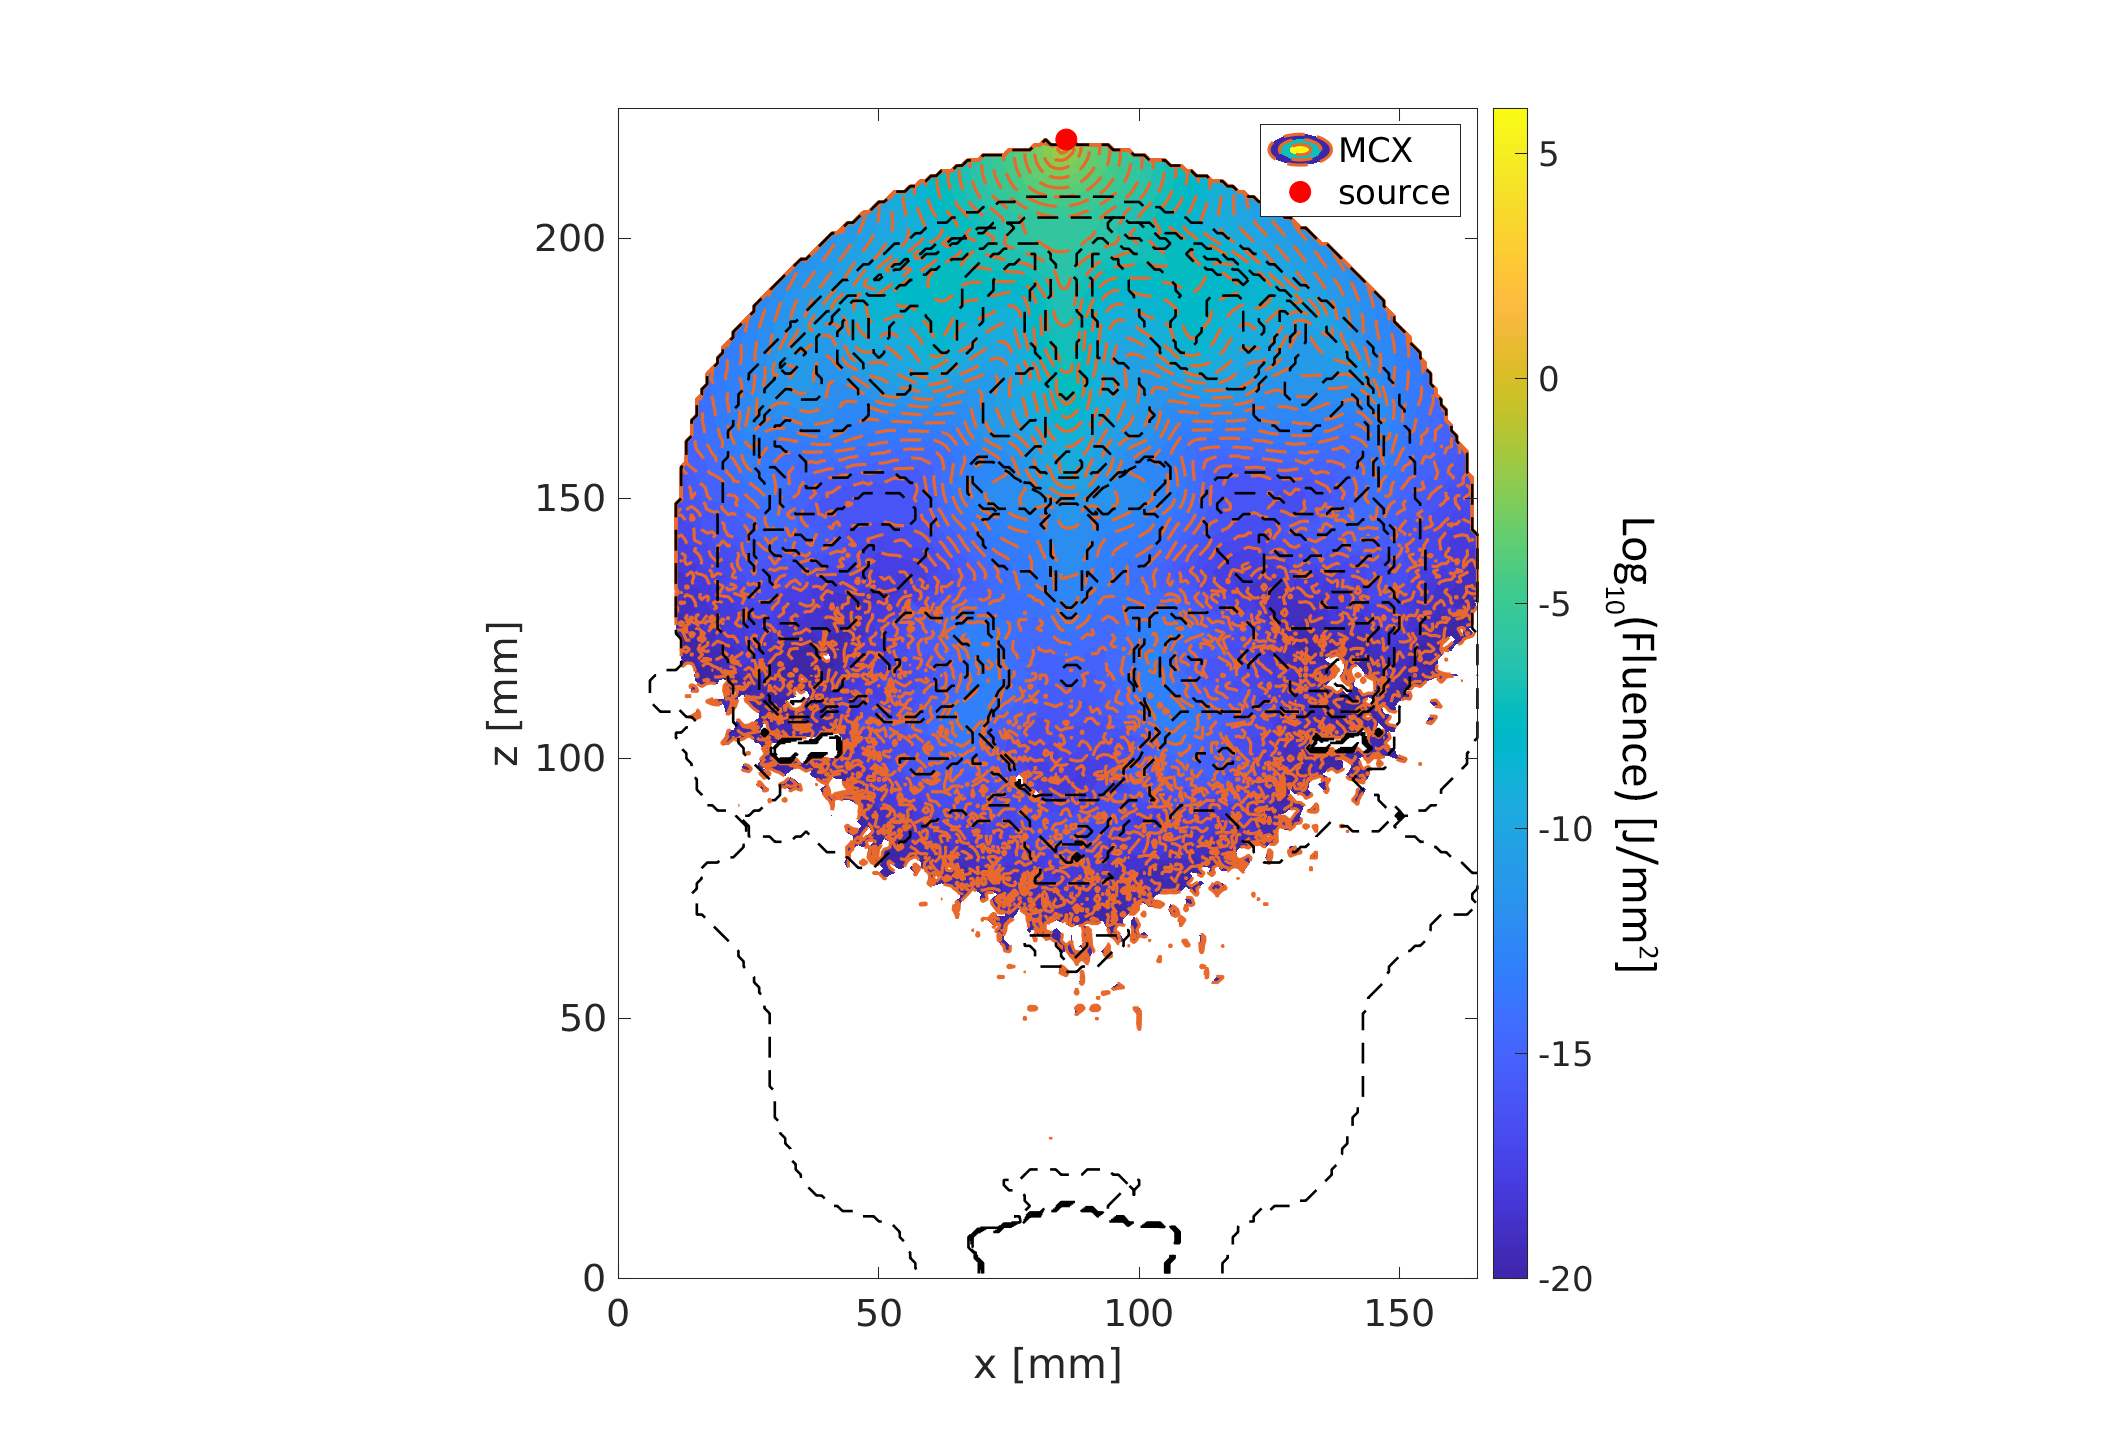
\includegraphics[width=\columnwidth]
    {Figures/Fluence_Distribution_1550nm_CZ.png}}
    \caption{\label{fig:1550-CZ} 1550 nm CZ Position}
\end{figure}

\begin{figure}[!htb]
    \center{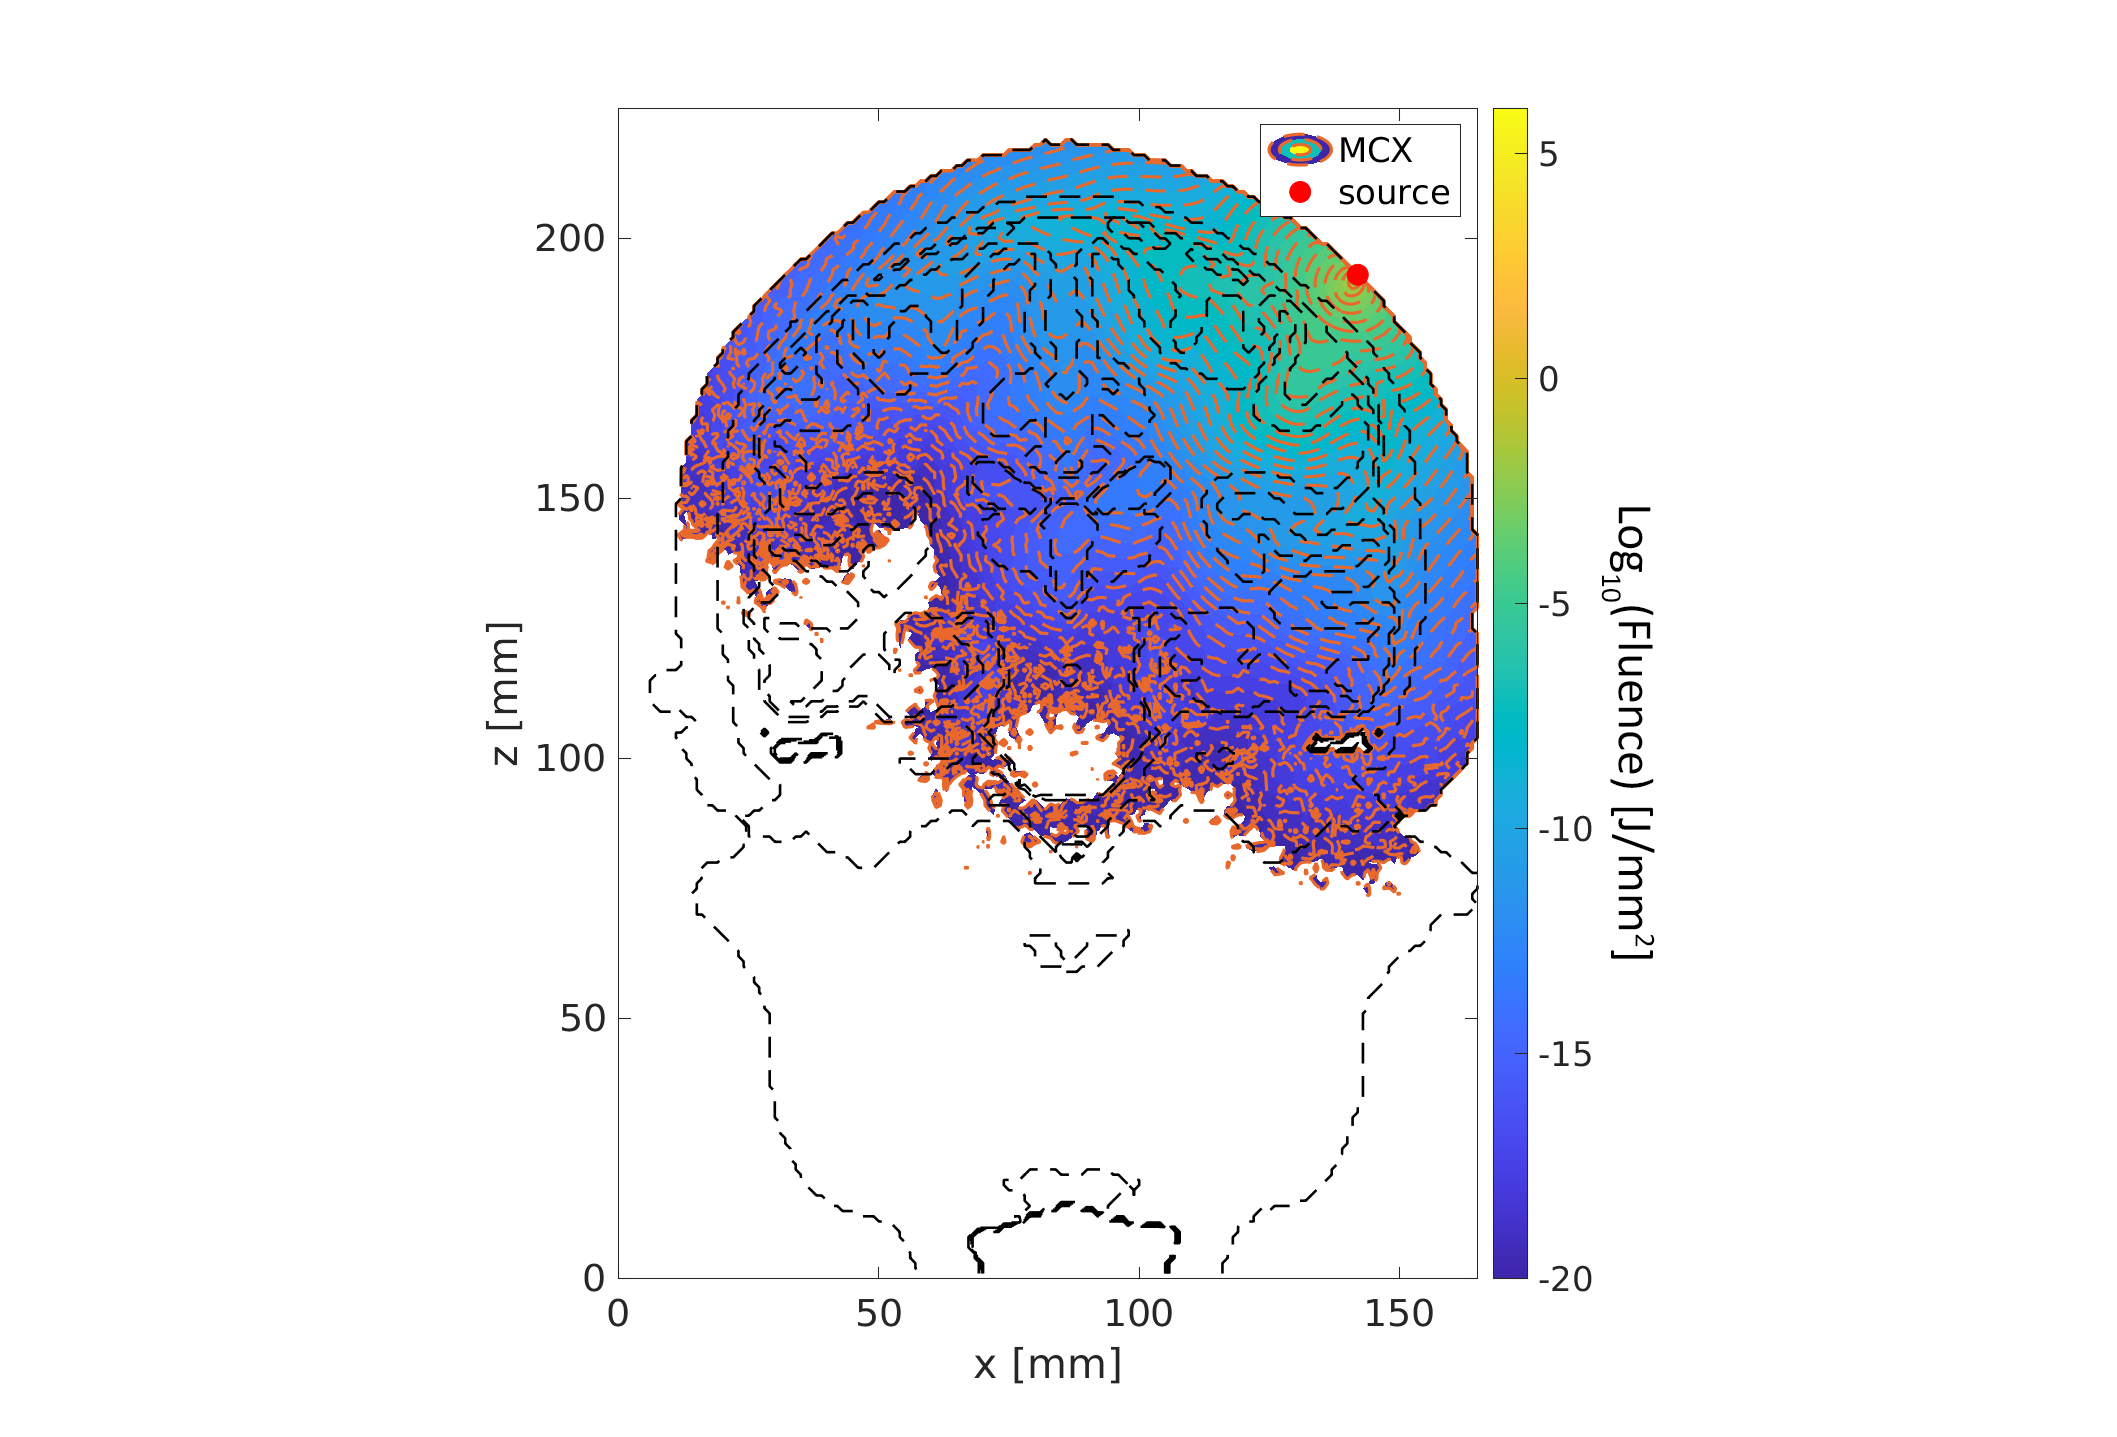
\includegraphics[width=\columnwidth]
    {Figures/Fluence_Distribution_1550nm_45deg.png}}
    \caption{\label{fig:1550-45} 1550 nm 45 Degree Position}
\end{figure}

\begin{figure}[!htb]
    \center{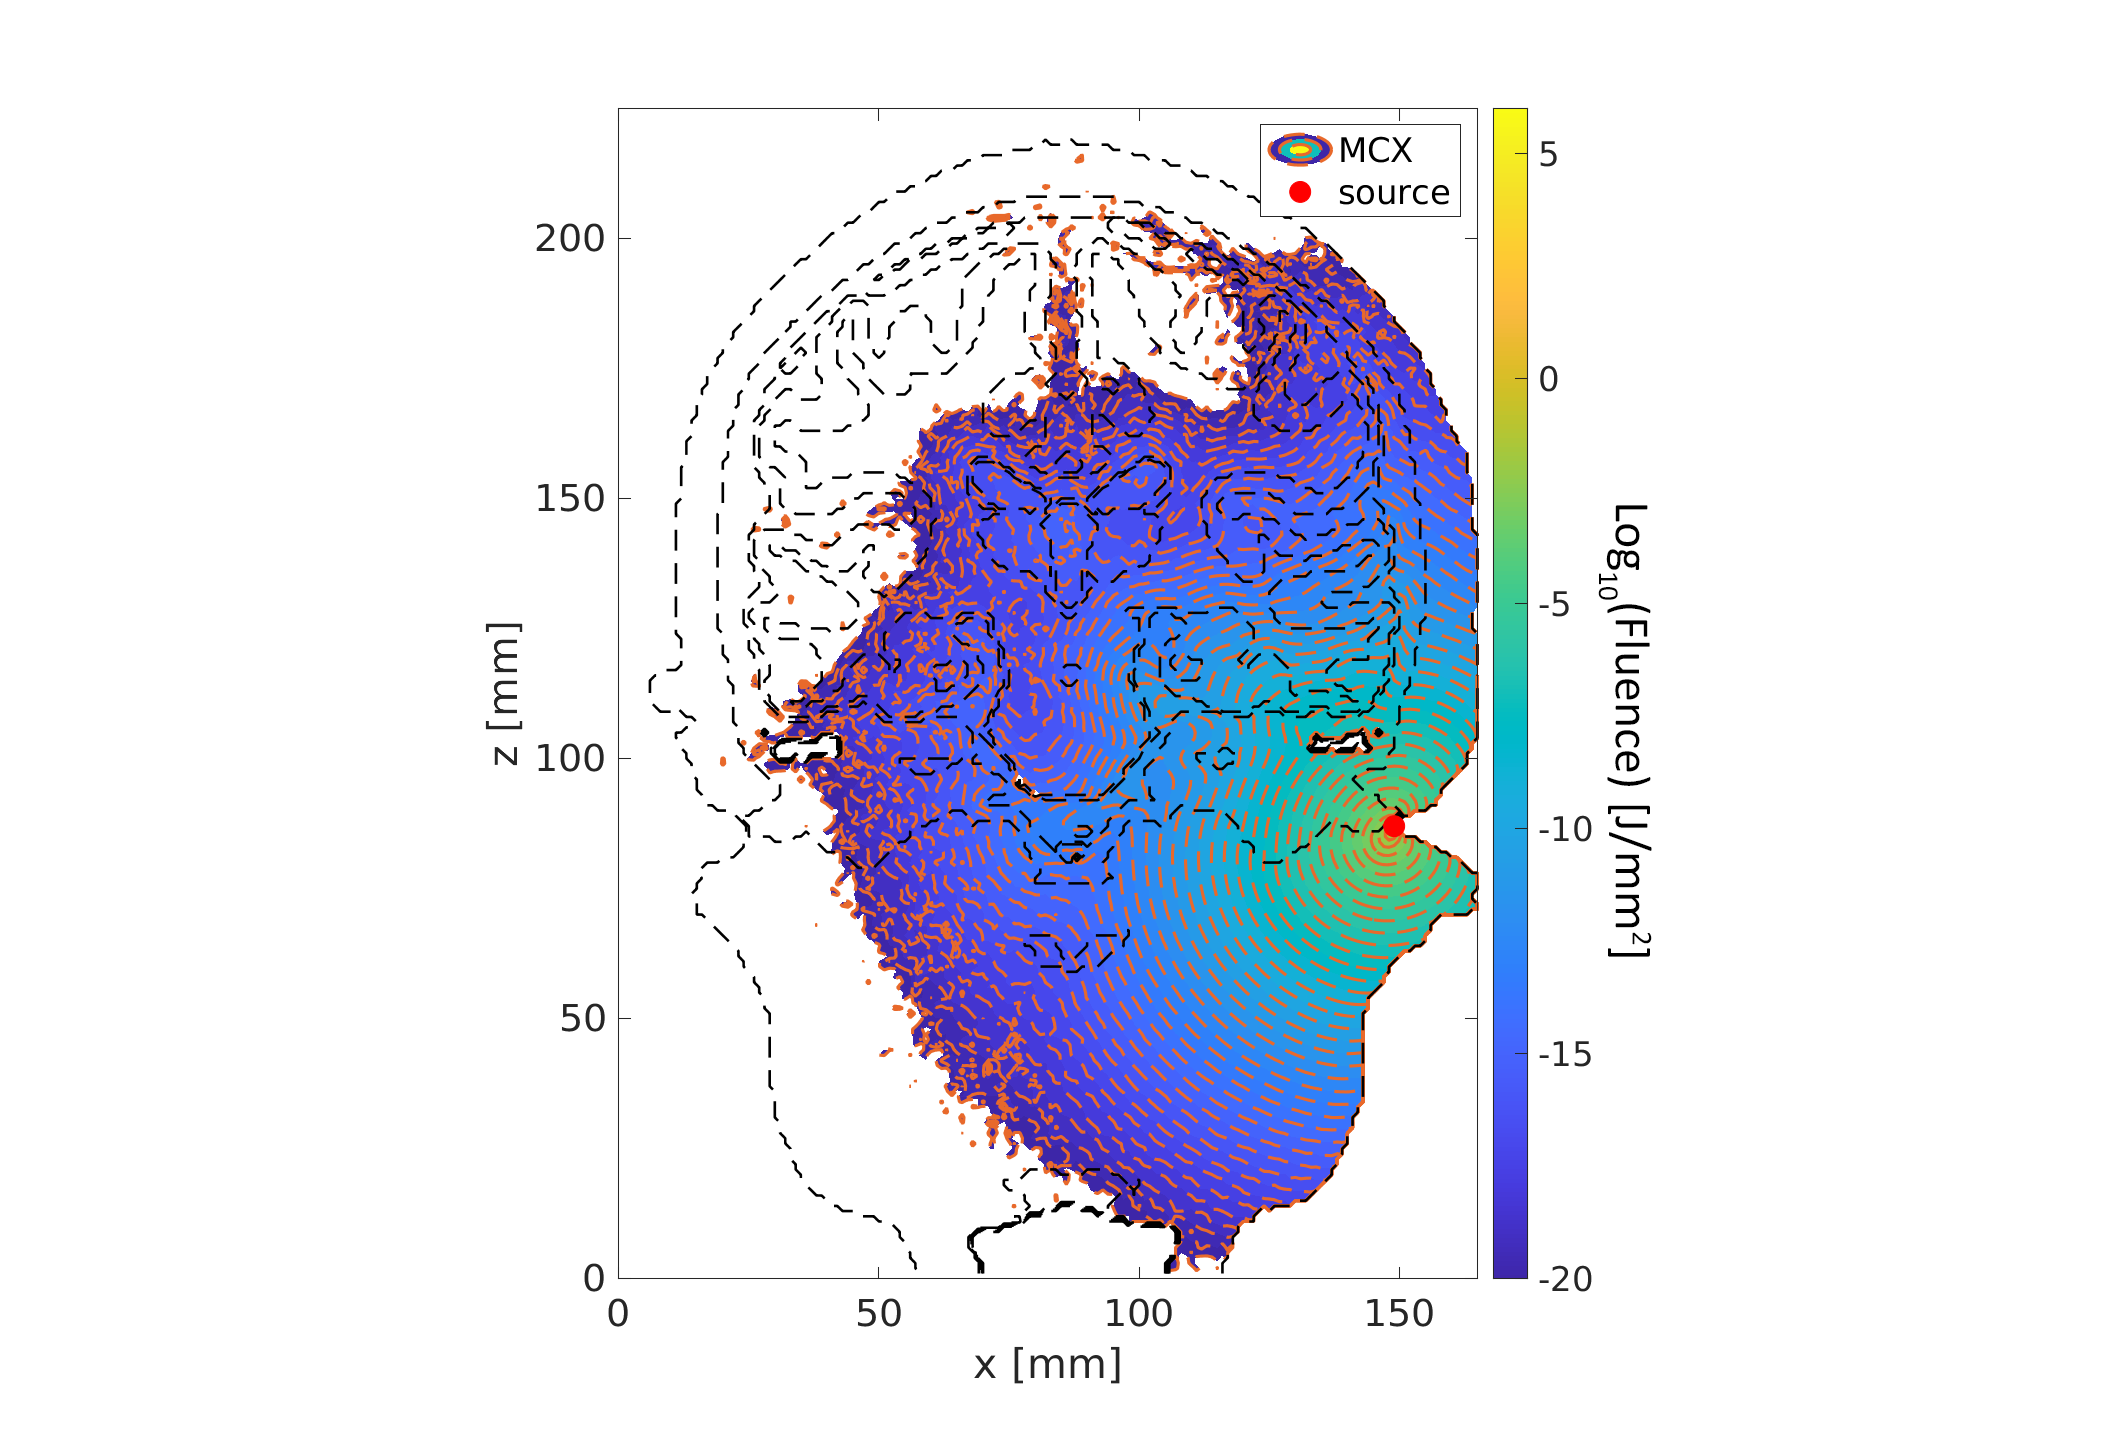
\includegraphics[width=\columnwidth]
    {Figures/Fluence_Distribution_1550nm_Cochlear.png}}
    \caption{\label{fig:1550-Cochlear} 1550 nm Cochlear Position}
\end{figure}

\begin{figure}[!htb]
    \center{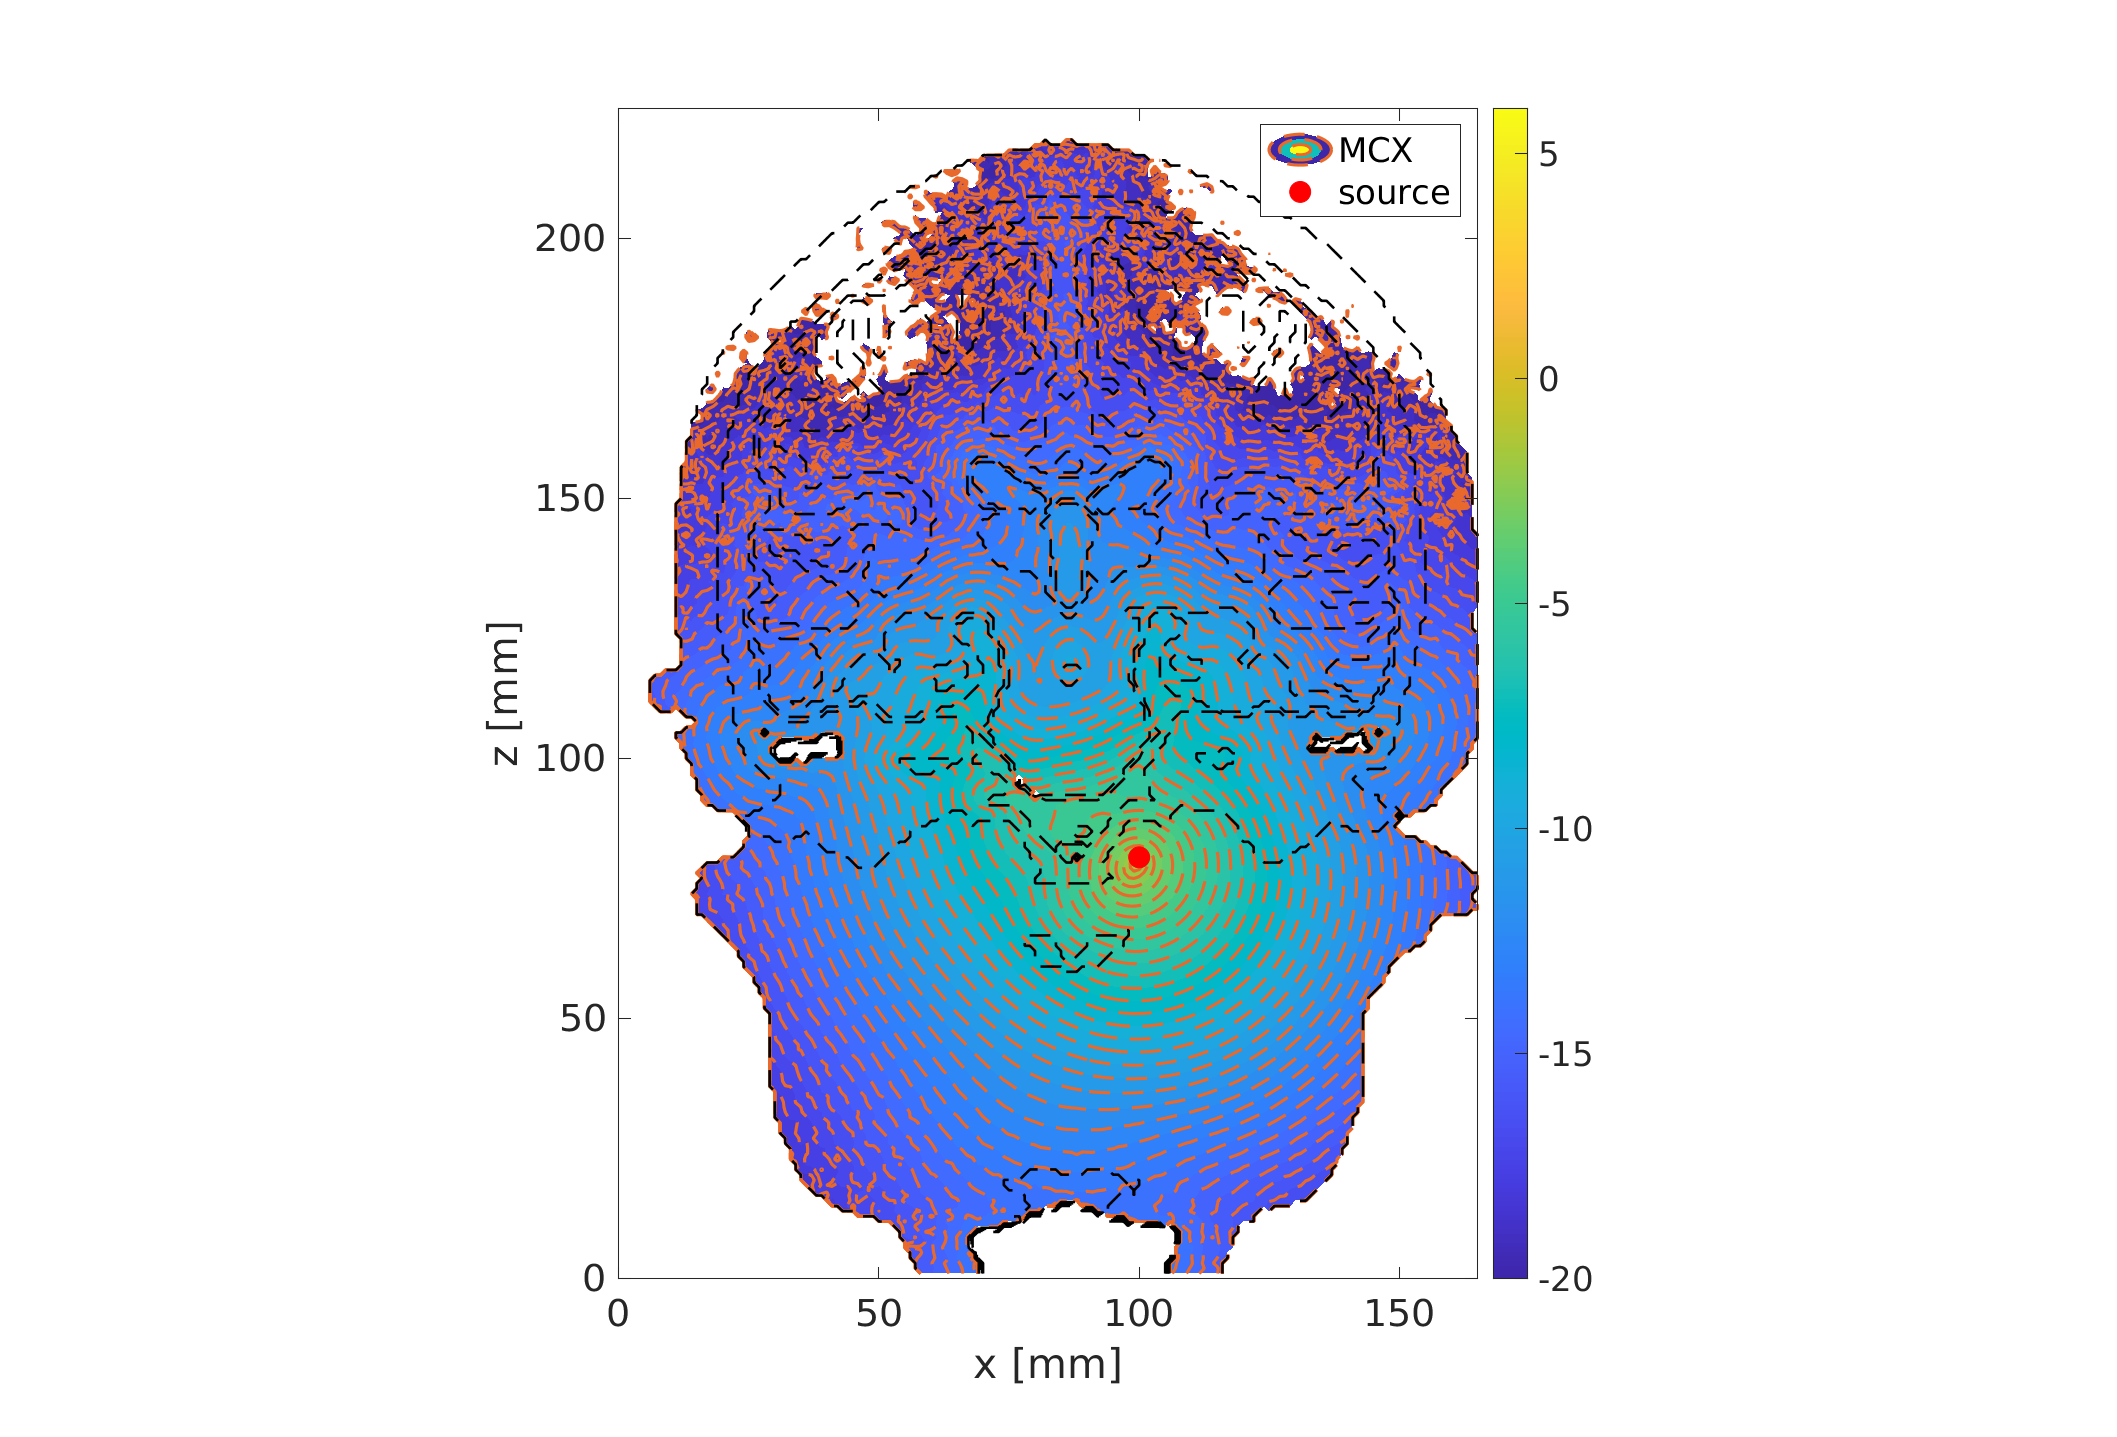
\includegraphics[width=\columnwidth]
    {Figures/Fluence_Distribution_1550nm_Intranasal.png}}
    \caption{\label{fig:1550-Intra} 1550 nm Intranasal Position}
\end{figure}

\section{Discussion}
\label{sec:next steps}

\section{Conclusion}
\label{sec:conclusion}

\section*{Acknowledgment}

\section*{References}

\end{document}
